\documentclass[12pt,a4paper,twoside,openright]{report}
\pagestyle{headings}


\def\magyarOptions{defaults=prettiest}
\usepackage[magyar]{babel}
\usepackage[latin2]{inputenc}
\usepackage[T1]{fontenc}
\usepackage{pslatex}
\usepackage{t1enc}

\usepackage{array}
\usepackage{amsmath}
\usepackage{amsfonts}
\usepackage{graphicx}
\usepackage[dvipdfm,bookmarks]{hyperref}
\usepackage{listings}
\usepackage{subfig}
\usepackage{stilus}

\newcommand{\urlszin}{blue}
\newcommand{\tobbiszin}{black}
\hypersetup{
  pdftitle={Haskell programok gr�f�t�r� rendszerr� transzform�l�sa},
  pdfauthor={Dollenstein Zsolt},
  pdfkeywords={haskell, gr�f�t�r� rendszer, diplomamunka},
  pdfstartpage=1,
  pdfmenubar=true,
  pdftoolbar=true,
  pdfstartview=FitH,
  bookmarksnumbered=true,
  bookmarksopen=false,
  bookmarksopenlevel=\maxdimen,
  pdfpagemode=UseNone,
  breaklinks=true,
  colorlinks=true,
  linkcolor=\tobbiszin,
  anchorcolor=\urlszin,
  citecolor=\tobbiszin,
  pagecolor=\tobbiszin,
  urlcolor=\urlszin
}

\frenchspacing

\hyphenation{}

\lstset{language=Haskell}


\begin{document}

\cleardoublepage
\thispagestyle{empty}



\newlength{\cimermeret}
\setlength{\cimermeret}{24mm}

\newlength{\seggmeret}
\setlength{\seggmeret}{\textwidth}
\addtolength{\seggmeret}{-\cimermeret}
\addtolength{\seggmeret}{-7mm}



\noindent
\begin{tabular}{p{\cimermeret}p{\seggmeret}}

\includegraphics[width=\cimermeret]{eps/eltecimer.eps}  &
\vspace{-17mm}
\begin{large}
\hspace*{\stretch{1}} E�tv�s Lor�nd Tudom�nyegyetem \hspace*{\stretch{1}} \newline
\hspace*{\stretch{1}} Informatikai Kar              \hspace*{\stretch{1}} \newline
\hspace*{\stretch{1}} Programoz�si Nyelvek �s       \hspace*{\stretch{1}} \newline
\hspace*{\stretch{1}} Ford�t�programok Tansz�k      \hspace*{\stretch{1}}
\end{large}                                             \\
\hline
\end{tabular}



\vspace{5cm}

\begin{center}
\begin{huge}
Gr�f�t�r� Rendszerr� Transzform�lt Haskell Programok Interpret�l�sa
\end{huge}
\end{center}



\vspace{3cm}

\noindent
Divi�nszky P�ter  \hspace*\fill  Dollenstein Zsolt               \\
\begin{small}
doktorandusz      \hspace*\fill  nappali tagozat            \\
                  \hspace*\fill  programtervez� matematikus \\
\end{small}



\vfill

\begin{center}
Budapest, 2009.
\end{center}



\clearpage
\thispagestyle{empty}
\cleardoublepage

%% Local Variables:
%% coding: latin-2
%% End:

\cleardoublepage


\begin{center}
\begin{scriptsize}
A diplomamunka bek�tve kell, hogy tartalmazza a kit�lt�tt �s j�v�hagyott diplomamunka
\textbf{t�mabejelent�t}. Ennek a lapnak a hely�re kell bek�tni.

\medskip
\csillagok
\end{scriptsize}
\end{center}


\cleardoublepage

%% Local Variables:
%% coding: latin-2
%% End:

\tableofcontents

\chapter{Bevezet�s}

Ebben a diplomamunk�ban gr�f�t�r� rendszerekkel foglalkozunk.

Ahhoz, hogy kit�zhess�k a c�lunkat, ismertet�nk p�r alapfogalmat a
gr�f�t�r� rendszerekkel kapcsolatban.

\csillagok

A gr�f�t�r�s (\emph{graph rewriting} vagy \emph{graph transformation})
azt a folyamatot jelenti, mely sor�n egy eredeti gr�fb�l valamilyen
automatizmus alapj�n egy �j gr�fot �ll�tunk el�. Form�lisan: egy
gr�f�t�r� rendszer $p : L \rightarrow R$ alak� szab�lyok halmaza, ahol
$L$ a minta gr�f (a szab�ly bal oldala), $R$ pedig a helyettes�t� gr�f
(a szab�ly jobb oldala).

A gr�f�t�r� rendszerek (melyeket el�sz�r \told{\cite{interm}}+ban{}
vezettek be) j�l haszn�lhat�ak valamilyen sz�m�t�s
modellez�s�re. Az �tlet az, hogy a sz�m�t�s egy adott �llapot�t
reprezent�ljuk egy gr�ffal. Egy adott �llapotb�l a k�vetkez�be �gy
jutunk, ha az eredeti �llapotnak megfelel� gr�fra alkalmazunk egy
szab�lyt, ez�ltal �j gr�fot (�llapotot) kapva. A szab�ly alkalmaz�sa
�gy t�rt�nik, hogy az eredeti gr�fra (vagy annak r�szgr�fj�ra)
illesztj�k a szab�ly bal oldal�t. Ezt a folyamatot mintailleszt�snek
h�vjuk.

Funkcion�lis nyelvek eset�n az�rt �rdemes gr�f�t�r� rendszerekkel
foglalkozni, mert ezek ismeret�ben a programoz� jobban �tl�tja a saj�t
k�dj�t, tudni fogja, hogy pontosan mi t�rt�nik a h�tt�rben a programja
fut�sa k�zben. Az adatgr�fok �s az �t�r�s folyamat�nak ismerete seg�t
megbecs�lni az adatcs�csok sz�m�t a program fut�sa k�zben, ami egyenes
ar�nyban �ll a sz�ks�ges mem�ri�val; illetve a (k�s�bb r�szletesen
t�rgyalt) redukci�s l�p�sek hasonl�k�ppen egyenes ar�nyban �llnak a
t�nyleges fut�si id�vel.

Ezt a modellt fogjuk haszn�lni a Haskell\footnote{Egy sokat aj�nlott
  bevezet� a nyelvbe, mely els�sorban azoknak sz�l, akik m�g nem
  tal�lkoztak funkcion�lis nyelvekkel: \cite{yaht}} eset�ben, ami egy lusta
funkcion�lis programoz�si nyelv\footnote{Egy bevezet� a nyelv 98-as
  verzi�j�ba (mely az 1998-ban kiadott szabv�nyt k�veti) olyanoknak,
  akik m�r tal�lkoztak legal�bb egy funkcion�lis nyelvvel:
  \cite{tutorial98}}. A lustas�g\footnote{A lustas�g
  megnyilv�nul�s�r�l a Haskell programoz�si nyelv eset�ben
  \acite{laziness} �r} ebben az esetben azt
eredm�nyezi, hogy k�nnyen, eleg�nsan tudunk kezelni v�gtelen
adatszerkezeteket an�lk�l, hogy ehhez k�l�n�sebb mem�ria vagy
h�tt�rt�r ig�nyeket t�masztan�nk. A gr�f�t�r� rendszerek seg�ts�g�vel
ilyen esetekben is j�l tudjuk modellezni a mem�ria- �s id�ig�nyt.

K�t f� fogalmat vezet�nk be.

\begin{definicio}[Adatgr�f]
  Adatgr�fnak nevezz�k azokat a gr�fokat, melyek teljes�tik a
  k�vetkez� krit�riumokat:
  \begin{itemize}
    \item ir�ny�tott
    \item l�tezik egy kit�ntetett cs�cs (gy�k�r), melyb�l b�rmelyik
      cs�cs el�rhet�
    \item minden cs�cshoz hozz� van rendelve egy szimb�lum
    \item egy adott cs�cs kimen� �lei sz�mozottak
  \end{itemize}
  Adatgr�f eset�n egy cs�cs �lein ezent�l a kimen� �leket �rtj�k.
\end{definicio}

Az egyszer�s�g kedv��rt minden adatgr�fnak defini�ljuk egy �gynevezett
sz�veges form�j�t, ami gyakorlatilag egy Haskell nyelven le�rt
kifejez�st jelent. Minden kifejez�shez tartozik egy olyan adatgr�f,
aminek az a kifejez�s a sz�veges form�ja. Ezzel meg is teremtett�k a
kapcsolatot a programsz�veg �s a gr�f�t�r� rendszer k�z�tt.

\begin{pelda}
  Vegy�k a k�vetkez� Haskell kifejez�st:
  \begin{lstlisting}
    l = [71, 72]
  \end{lstlisting}
  Ez defini�l egy $l$ szimb�lumot, melyhez egy k�t elem� list�t k�t,
  melynek elemei rendre $71$ �s $72$. Ez az �r�sm�d tulajdonk�ppen egy
  szintaktikus egyszer�s�t�se a megfelel� list�nak:
  \begin{lstlisting}
    [71, 72] == 71 : 72 : []
  \end{lstlisting}
  Az egyenl�s�g jobb oldal�n tal�lhat� kifejez�s mutatja, hogyan
  reprezent�lja a list�kat a nyelv specifik�ci�ja. K�t konstruktort
  figyelhet�nk meg: a $(:)$  ,,listab�v�t� oper�tort'', mely a
  baloldali argumentum�t (egy elem) a jobboldali argumentuma (egy
  lista) el� helyez; valamint a $[]$ �res lista konstruktort. A fenti
  kifejez�shez tartoz� adatgr�fot \aref{fig:lstdatag}. �bra mutatja.
  \begin{figure}[htb]
    \begin{center}
      \caption{Egy k�telem� list�hoz tartoz� adatgr�f \label{fig:lstdatag}}
      \includegraphics[height=0.3\textheight]{eps/grw_5.eps}
    \end{center}
  \end{figure}
\end{pelda}

Az adatgr�fok nagy ereje abban rejlik, hogy tudunk vel�k �gynevezett
\emph{megosztott kifejez�seket} �br�zolni. Ez azt jelenti, hogy ha
p�ld�ul k�tszer kell felhaszn�lnunk egy kifejez�sben egy
r�szeredm�nyt, az nem kell, hogy k�tszer szerepeljen az
adatgr�fban. M�sk�ppen megfogalmazva: a r�szeredm�nyeket el tudjuk
t�rolni adatgr�fokn�l.

\begin{pelda}
  N�zz�nk teh�t egy olyan kifejez�st, amin�l hasznos lehet a
  r�szeredm�nyek elt�rol�sa. Egy egyszer� p�lda erre a
  \begin{verbatim}
    (5+5)! * (5+5)!
  \end{verbatim}
  kifejez�s, melyben k�tszer lehetne kisz�molni az �tnek �s az �tnek
  az �sszeg�t, majd ennek a faktori�lis�t. N�zz�k teh�t ezt
  k�tf�lek�ppen adatgr�fk�nt �br�zolva: a r�szeredm�nyek elt�rol�s�t
  \aref{fig:sharingyes} �bra mutatja, m�g a naiv megold�st
  \aref{fig:sharingno} �bra.

  \begin{figure}[htb]
    \begin{center}
      \caption{Az (5+5)! * (5+5)! kifejez�s adatgr�fjai \label{fig:sharing}}
      \captionsetup{position=top}
      \subfloat[Megoszt�s n�lk�l]{
        \label{fig:sharingno}
        \includegraphics[height=0.3\textheight]{eps/sharing1.eps}
      }
      \vrule
      \subfloat[Megoszt�ssal]{
        \hspace{1cm}
        \label{fig:sharingyes}
        \includegraphics[height=0.3\textheight]{eps/sharing2.eps}
      }
    \end{center}
  \end{figure}
\end{pelda}

\begin{definicio}[Redukci�]
  A gr�fredukci� sor�n egy az adatgr�fban tal�lhat� szimb�lumot
  helyettes�tj�k egy megfelel� �t�r�si szab�ly �ltal el��rt m�sik
  szimb�lummal (vagy szimb�lumokkal).
\end{definicio}

Az �t�r�si szab�lyokat a programban tal�lhat� f�ggv�nyek defin�ci�i
adj�k. Egy redukci�s l�p�s sor�n teh�t egy f�ggv�ny szimb�lumot
(�s argumentumait) helyettes�tj�k a f�ggv�ny t�rzs�vel. Egy
redukci�s l�p�s csak egyetlen f�ggv�ny szimb�lumot elimin�l, viszont
term�szetesen a t�rzs tartalmazhat �jabb f�ggv�ny h�v�sokat.

\begin{pelda}
  Term�szetesen egy f�ggv�ny defin�ci�j�t k�t r�szre lehet bontani. A
  bal oldal (\emph{left hand side}, \emph{lhs}) megadja a f�ggv�ny
  nev�t, illetve az argumentumait --- a Haskell eset�ben mint�kat,
  melyeket k�s�bb illeszteni lehet konkr�t argumentumokra. A jobb
  oldal (\emph{right hand side}, \emph{rhs}) pedig maga a
  f�ggv�nyt�rzs, melyben le�rjuk, hogy a jobb oldalon megadott
  mintailleszt�sek ut�n a f�ggv�ny szimb�lumot �s argumentumait milyen
  kifejez�sre kell lecser�lni. Ez j�l megfeleltethet� az �t�r�si
  szab�lyok bal- �s jobb oldal�nak, �s val�ban ez �ll a defin�ci�
  h�tter�ben.
  A k�vetkez� egyszer� f�ggv�ny a logikai \emph{�s} m�veletet val�s�tja
  meg:
  \begin{lstlisting}
    False && _ = False
    True  && a = a
  \end{lstlisting}
  Ebb�l a k�dr�szletb�l k�t �t�r�si szab�ly keletkezik --- soronk�nt
  egy.
  L�that�, ahogy az els� szab�lyban k�t k�l�nb�z� cs�csba ugyanaz a
  (\emph{False}) �rt�k �r�dott. Ez azt jelenti, hogy a ki�rt�kel�s
  k�zben k�tszer t�rol�dik el ez az �rt�k (egyszer a
  mintailleszt�sn�l, egyszer a szab�ly jobb oldal�n�l). Ezen persze
  lehet jav�tani Haskell-ben a k�vetkez� megold�ssal:
  \begin{lstlisting}
    f@False && _ = f
  \end{lstlisting}
  Itt az \emph{f} szimb�lum egy referencia lesz arra a kifejez�sre,
  ami illeszkedett a \emph{False} konstruktorra. Az �gy kialakult
  szab�ly hasonl�t \aref{fig:esmasodik} �br�ra.

  \begin{figure}[htb]
    \captionsetup{position=top}
    \captionsetup[subfloat]{captionskip=-20pt}
    \caption{A logikai \emph{�s} k�t szab�lya}
    \begin{center}
      \subfloat[Els� sor\label{fig:eselso}]{
        \includegraphics{eps/grw_14.eps}
        \captionsetup{position=top}
      }
      \subfloat[M�sodik sor\label{fig:esmasodik}]{
        \captionsetup{position=top}

        \includegraphics[height=7cm]{eps/grw_15.eps}
      }
      \vspace{28pt}
    \end{center}
    \label{fig:esszabaly}
  \end{figure}


  A m�sodik szab�ly arra mutat p�ld�t, hogy a bal oldalon kialakult
  k�t�seket haszn�lhatjuk a jobb oldalon is, s�t, hat�konys�gi okokb�l
  �rdemes is ezt tenni.
\end{pelda}

Ezen diplomamunk�hoz tartoz� program egy Haskell nyelven �r�dott
programsz�veget transzform�l gr�f�t�r� rendszerr�, majd ebben a
gr�f�t�r� rendszerben egy tetsz�leges Haskell kifejez�s �t�r�si
l�p�seit hajtja v�gre, illetve rajzolja ki a k�perny�re. Egy tov�bbi
funkci�val is rendelkezik, mellyel mag�t a gr�f�t�r� rendszert
jelen�thetj�k meg, pontosabban a rendszerben tal�lhat� szab�lyok jobb
oldal�t. A kiv�lasztott funkci�t�l f�gg�en a felhaszn�l� interakt�van
l�pkedhet az els� esetben az �t�r�si l�p�sek k�z�tt, a m�sodikban
pedig a szab�lyok k�z�tt el�re-h�tra. A program c�lja az, hogy egy
olyan eszk�zt biztos�tson, amivel k�nnyebben �rthet�ek lesznek
egyszer�, Haskell nyelven �rt funkcion�lis k�dok, ez�ltal seg�thet a
teljes�tm�ny elemz�sben, illetve azoknak, akik �pp ismerkednek a
funkcion�lis programoz�s rejtelmeivel.

A dolgozat h�tralev� r�sz�ben el�sz�r ismertetj�k a gr�f�t�r�
rendszerek elm�leti alapjait, majd a konkr�t implement�ci�s
megfontol�sokra t�r�nk r�.

%% Local Variables:
%% coding: latin-2
%% End:


% LocalWords:  rewriting transformation left hand side lhs right rhs False pt
% LocalWords:  position subfloat captionskip esmasodik

\chapter{Elm�leti alapok}

Ebben a fejezetben a gr�f�t�r� rendszerek elm�leti alapjaival
foglalkozunk. A form�lis defin�ci�khoz sz�ks�ges szintaktika
az egyszer�s�g �s �rthet�s�g kedv��rt megegyezik a \cite{cleanbook}
jel�l�seivel.

\section{Adatgr�fok}

A bevezet�ben t�rgyalt defin�ci�ja az adatgr�foknak egy j� k�pet ad
arr�l, hogy mi�rt is fontos ez a fogalom. Ebben a pontban egy pontos,
matematikailag prec�z defin�ci�t adunk r�juk, megadjuk a kanonikus
alakjukat, egy r�vid�tett le�r�si form�t, illetve egy�b fontos
tulajdons�gaikat.

Az egyik f� c�l az adatgr�fok defin�ci�j�n�l, hogy k�pesek legyenek
reprezent�lni a bevezet� utols� p�ld�j�ban le�rt referencia
konstrukci�t. Ez az�rt hasznos, hogy el tudjuk ker�lni egy adott
sz�m�t�s t�bbsz�ri ki�rt�kel�s�t, �s a m�r esetleg kisz�molt eredm�nyt
�jra fel tudjuk haszn�lni. Ezt a technik�t a sz�m�t�sok megoszt�s�nak
(\emph{sharing}) h�vjuk.

\subsection{Szintaxis}

Egy gr�f�t�r� rendszerben az adatgr�fokat k�tf�lek�ppen �rhatjuk le:
kanonikus form�ban �s r�vid�tett form�ban. Ez ut�bbi eset l�nyege,
hogy nem kell teljesen specifik�lni a gr�f strukt�r�j�t, �pp csak
annyit, hogy egy�rtelm�en ki lehessen k�vetkeztetni azt a le�r�sb�l. A
kanonikus forma eset�ben ezzel ellent�tben az eg�sz strukt�r�t
r�szletesen specifik�lni kell. �ltal�ban a r�vid�tett form�t
haszn�ljuk az �tl�that�s�ga miatt. Fontos megjegyezni, hogy a
r�vid�tett le�r�sb�l term�szetesen el��ll�that� a kanonikus alak,
ekkor pedig a k�t le�r�s pontosan ugyanazt az adatgr�fot jel�li, teh�t
az egyiket minden tov�bbi n�lk�l lehet haszn�lni a m�sik helyett.

A gr�f specifik�ci�j�hoz minden esetben sz�ks�g�nk lesz egy konstans
szimb�lumokb�l (nem �res sztringek, melyek nagybet�vel kezd�dnek)
�ll�, valamint egy cs�cs azonos�t�kb�l (kisbet�vel kezd�d� nem �res
sztringek) �s cs�cs konstansokb�l (a ,,@'' kukac karakterrel kezd�d�
sztringek) �ll� halmazra.

\subsubsection{Kanonikus alak}

Egy adatgr�f kanonikus alakj�t a k�vetkez� szintaxissal defini�ljuk:

\begin{align*}
  \tt{Graph}   &= \tt{NodeDef} \hogy \tt{NodeDef} \lit{,} \tt{Graph} \\
  \tt{NodeDef} &= \tt{Nodeid} \lit{:} \tt{Node} \\
  \tt{Node}    &= \tt{Symbol} \{\tt{Arg}\} \hogy \tt{EmptyNode} \\
  \tt{Symbol}  &= \predef{Constant} \\
  \tt{Arg}     &= \tt{Nodeid} \\
  \tt{Nodeid}  &= \predef{NodeidVariable} \hogy \predef{NodeidConstant} \\
  \tt{EmptyNode} &= \lit{$\mathbf{\bot}$}
\end{align*}

Egy adatgr�f teh�t cs�cs defin�ci�k (\tt{NodeDef}) egy halmaza. A
gr�fban minden cs�cshoz tartozik egy egyedi azonos�t� (\tt{Nodeid}),
mely vagy ,,@''-cal kezd�dik (\predef{NodeidConstant} -- konstans),
vagy kisbet�vel (\predef{NodeidVariable} -- v�ltoz�). Egy cs�cs
defin�ci�j�hoz (\tt{NodeDef}) kell egy ilyen cs�cs azonos�t�, majd
egy ,,:'' karakter ut�n k�vetkezik a cs�cs le�r�sa
(\tt{Node}). Minden cs�cshoz tartozik egy konstans szimb�lum
(\tt{Symbol}), melynek esetleg argumentumai (\tt{Arg})
lehetnek. Ezek az argumentumok tulajdonk�ppen cs�cs azonos�t�k, melyek
defini�lj�k az �leket a gr�f �br�zolt form�j�ban.

\begin{pelda}
  \Aref{fig:lstdatag}. �br�n tal�lhat� adatgr�f kanonikus alakja (a
  $(:)$ konstruktornak most a k�t param�teres \con{Cons}, a $[]$
  konstruktornak pedig a \con{Nil} felel meg):

  \begin{canonDG}
      \cn{1} & \con{Cons} \cn{2} \cn{3}, \\
      \cn{2} & 71, \\
      \cn{3} & \con{Cons} \cn{4} \cn{5}, \\
      \cn{4} & 72, \\
      \cn{5} & \con{Nil} \\
  \end{canonDG}

  Itt teh�t nincsenek v�ltoz� cs�cs azonos�t�k, csak konstansok (\cn{1}
  \ldots \cn{5}), valamint a konstans szimb�lumok a k�vetkez�k:
  \con{Cons}, 71, 72, \con{Nil}.
\end{pelda}

\subsection{Szemantika}

Az adatgr�fok szemantik�j�t a kanonikus alakjuk figyelembev�tel�vel,
azok alapj�n fogjuk megadni.

Minden adatgr�fnak l�tezik egy kit�ntetett cs�csa, melyet a gr�f
\emph{gy�ker�}nek h�vunk. A kanonikus alakban mindig ezt a cs�csot
soroljuk fel el�sz�r. Egy adatgr�f \emph{r�szgr�f}j�nak kanonikus
alakja az eredeti gr�f kanonikus alakj�ban tal�lhat� cs�cshalmaz
r�szhalmaz�b�l �ll. Egy \emph{�t} a gr�fban olyan cs�cs azonos�t�k
sorozata, melyben az els� kiv�tel�vel minden azonos�t� a k�zvetlen�l
megel�z� azonos�t�hoz tartoz� cs�cs egyik argumentuma. Az �t $A$-b�l
$B$-be megy, ha $A$ azonos�t�ja az els�, $B$ azonos�t�ja pedig az
utols� a sorozatban. A gr�fban \emph{k�r}nek h�vjuk azokat az utakat,
melyeknek ugyanaz az els� �s az utols� cs�cs azonos�t�juk. A gr�f
k�rmentes, ha nincs benne k�r. Egy $B$ cs�cs \emph{el�rhet�} $A$-b�l,
ha l�tezik a gr�fban �t $A$-b�l $B$-be. Ha minden cs�cs el�rhet� a
gy�k�rb�l, akkor a gr�f \emph{�sszef�gg�}. Egy adatgr�fot
\emph{z�rt}nak h�vunk, ha nincs benne v�ltoz� cs�cs azonos�t�,
egy�bk�nt \emph{ny�lt}nak. Egy gr�f $n$ \emph{cs�cst�l kezd�d�
  r�szgr�fja} az a $g$ �sszef�gg� r�szgr�f, melynek gy�kere $n$, �s
tartalmazza mindazokat a cs�csokat, melyek el�rhet�ek $n$-b�l.

\begin{megj}
  Tartsuk szem el�tt, hogy az adatgr�fokn�l egy �thoz tartozik annak
  egy ir�ny�t�sa is, teh�t a k�r�kn�l, illetve az �sszef�gg�s�gn�l is
  figyelembe kell venni ezt az ir�ny�t�st. Ez a fogalomrendszer nagyon
  hasonl�t az ir�ny�tott gr�fokn�l szok�soshoz, tulajdonk�ppen itt is
  err�l van sz�, mint azt a bevezet�ben eml�tett�k.
  Megjegyzend� tov�bb�, hogy gr�f�t�r� rendszerekben az �sszes gr�f,
  bele�rtve a szab�lyokat is, mindig �sszef�gg�.
\end{megj}

\begin{pelda}
 \Aref{fig:lstdatag}. �br�n l�that� adatgr�f p�ld�ul �sszef�gg�, de
 k�rmentes �s z�rt.

 \begin{figure}[htb]
   \begin{center}
     \caption{Egy v�gtelen hossz�, v�gtelen�l egyszer� lista
       adatgr�fja \label{fig:inflist}}
     \includegraphics[height=0.3\textheight]{eps/grw_new_28.eps}
   \end{center}
 \end{figure}
 \Aref{fig:inflist}. �br�n tal�lhat� adatgr�f a v�gtelen hossz�, csupa
 tizenegyeseket tartalmaz� list�hoz tartozik. Kanonikus alakja:

 \begin{canonDG}
   \cn{1} & \con{Cons} \cn{2} \cn{1}, \\
   \cn{2} & 11
 \end{canonDG}

 Ez a gr�f l�that� m�don
 v�ges (mint minden adatgr�f), z�rt, �sszef�gg�, �s tartalmaz egy k�rt
 (teh�t hurok�leket term�szetesen megenged�nk). Ebb�l a p�ld�b�l is
 l�tszik a gr�f�t�r� rendszerek (�s azon bel�l egyel�re az adatgr�fok)
 kifejez�ereje.
\end{pelda}

\begin{figure}[bh]
  \begin{center}
    \caption{Ekvivalens gr�fok k�zti izomorfizmus \label{fig:grafekvizo}}
    \includegraphics[width=14cm]{eps/graf_ekv_izo.eps}
  \end{center}
\end{figure}

K�t z�rt gr�fot \emph{ekvivalens}nek nevez�nk, ha a cs�cs
azonos�t�kt�l eltekintve azonosak. Ez azt jelenti, hogy a k�t gr�fnak
ugyanaz a strukt�r�ja, �s a megfelel� cs�csok ugyanazokat a
szimb�lumokat tartalmazz�k. Form�lisan, l�tezik egy $\varphi :
\text{NodeidConstant} \rightarrow \text{NodeidConstant}$ bijekci�,
melyet ha alkalmazunk az egyik gr�f kanonikus alakj�ban tal�lhat�
cs�cs azonos�t�kra, akkor a m�sik gr�f kanonikus alakj�t
kapjuk. Figyelembe v�ve azt, hogy az adatgr�f �s a kanonikus alakja
k�z�tt is megadhat� egy bijekci�, ebb�l k�vetkezik, hogy ha k�t gr�f
ekvivalens, akkor l�tezik k�zt�k gy�k�rtart� izomorfizmus. Ezt a
gondolatmenetet v�zolja \aref{fig:grafekvizo}. �bra.

\section{�t�r� rendszerek}

Egy gr�f�t�r� rendszer l�nyege az, hogy j�l defini�lt m�don tudjunk
adatgr�fokat manipul�lni. A rendszer �t�r�si szab�lyok halmaza,
melyeket hasonl�an fogunk megk�zel�teni, mint fentebb az adatgr�fokat:
el�sz�r defini�ljuk a kanonikus alakjukat, ezzel szintaxist adva a
gr�f�t�r� rendszereknek, majd megadjuk a hozz�juk tartoz� szemantik�t.

\subsection{Szintaxis}

Ebben az alpontban megadjuk a gr�f�t�r� rendszerek kanonikus alakj�t,
majd egy p�ld�val r�mutatunk, hogy mennyire k�nyelmetlen ebben a
form�ban kezelni azokat, �gyhogy megadunk egy r�vid�tett form�t is.

\subsubsection{Kanonikus alak}

A gr�f�t�r� rendszerek szintaxisa teh�t a k�vetkez�k�ppen �rhat� le:

\begin{align*}
  \tt{CanonicalGRS} &= \tt{Rule} \hogy \tt{Rule} \tt{CanonicalGRS}\\
  \tt{Rule} &= \tt{RedexPattern} \lit{$\rightarrow$} \{\tt{Contractum}\} \tt{Redirection} \\
  \tt{Contractum} &= \tt{ContractumPattern} \\
  &\hogy \tt{ContractumPattern} \lit{,} \tt{Contractum} \\
  \tt{RedexPattern} &= \predef{Graph} \\
  \tt{ContractumPattern} &= \predef{Graph} \\
  \tt{Redirection} &= \predef{Nodeid} \lit{$\mathbf{\leftarrow}$} \predef{Nodeid}
\end{align*}
Ahol a \predef{Nodeid} �s a \predef{Graph} defin�ci�ja az adatgr�fokn�l
megadottal egyezik meg. A fenti defin�ci�b�l is l�tszik, hogy a
szab�lyok az $r : \alpha_r \rightarrow \beta_r, \varphi_r$ alakot
k�vetik, ahol $\beta_r$ opcion�lis. Ebben a jel�l�sben az $\alpha_r$-t
nevezik \emph{redex mint�}nak (ami a \emph{reducible expression}, azaz
 reduk�lhat� kifejez�s, angol sz�fordulatb�l sz�rmazik)
 a nem k�telez� $\beta_r$ neve
\emph{csere minta}\footnote{A t�bl�zatokban a csere minta angol
  megfelel�je, a contractum pattern szerepel}, a $\varphi_r$ pedig az
�tir�ny�t�s vagy \emph{redirekci�}.

Egy szab�lyban minden cs�cs azonos�t� legfeljebb egyszer lehet
defini�lva, illetve a jobb oldalon szerepl� azonos�t�khoz kell
tartozzon ugyanezen a jobb oldalon defin�ci� vagy szerepelni�k kell a
bal oldalon. A redirekci� bal oldal�n tal�lhat� azonos�t�nak mindig
meg kell egyeznie a redex minta gy�ker�vel (pontosabban annak
azonos�t�j�val), a jobb oldali cs�cs azonos�t� pedig vagy a csere
minta gy�kere, vagy egy olyan azonos�t�, ami szerepel a redex
mint�ban.

Az els� szimb�lumot a redex mint�ban \emph{f�ggv�ny szimb�lum}nak
h�vjuk. Az a szimb�lum, mely egyik minta els� elemek�nt se szerepel, a
\emph{konstruktor szimb�lum}. Term�szetesen f�ggv�ny szimb�lumok nem
csak a minta fej�ben szerepelhetnek, hanem b�rhol m�shol a mint�ban.

\begin{pelda}
  A k�vetkez� p�r sor Haskell k�d defini�l egy olyan f�ggv�nyt,
  melynek neve \emph{head}, �s
  egy lista els� elem�t adja vissza\footnote{Figyelj�k meg, hogy �res
    list�ra nincs defini�lva a \emph{head} f�ggv�ny. Ez nem probl�ma
    eg�szen addig, am�g �res list�ra nem pr�b�ljuk
    illeszteni. Haskell-ben ekkor egy programhiba �zenetet kapunk, az
    elm�letben viszont egyszer�en nem illeszkedik ilyen esetben a
    szab�ly}, egy defin�ci� szerint (a szok�sos m�don) rekurzi�val
  megval�s�tott faktori�lis f�ggv�nyt, illetve egy kezd�szimb�lumot,
  mely a k�s�bbiekben a gr�f�t�r�s kezd�pontja lesz.
  \begin{lstlisting}
    head (a:b) = a
    fact 0 = 1
    fact n = n * fact (n-1)

    start = fact (head [1000])
  \end{lstlisting}
  Ebb�l a p�r sorb�l fel�rhatunk egy olyan gr�f�t�r� rendszert,
  melyben n�gy szab�ly van (minden sornak megfelel egy, figyelj�k meg,
  hogy a faktori�lis f�ggv�nyhez tartoz� k�t sorb�l is k�t k�l�n
  szab�ly keletkezik). Ennek a rendszernek a kanonikus alakja a k�vetkez�:
  \begin{canonGRS}
    r:~\con{Head}~x, \n
    x:~\con{Cons}~a~b & \rightarrow & r \leftarrow a \n
    \n
    r:~\con{Fact}~x, \n
    x:~0 & \rightarrow & r':~1, ~ r \leftarrow r' \n
    \n
    r:~\con{Fact}~n & \rightarrow & r':~*~n~u, \n
    & & u:~\con{Fact}~v, \n
    & & v:~-~n~w, \n
    & & w:~1, \n
    & & r \leftarrow r' \n
    \n
    r:~\con{Start} & \rightarrow & r':~\con{Fact}~a,\n
    & & a:~\con{Head}~b, \n
    & & b:~\con{Cons}~c~d,\n
    & & c:~1000,\n
    & & d:~\con{Nil} \n
    & & r \leftarrow r' \n
  \end{canonGRS}
\end{pelda}

\subsubsection{R�vid�tett alak}

Mint a fenti p�ld�kb�l l�that�, az adatgr�fok �s a gr�f�t�r�
rendszerek kanonikus alakj�t neh�zkes olvasni, bonyolultabb esetekben
sok benne a redund�ns inform�ci�. Ez adja a motiv�ci�t ahhoz, hogy
defini�ljuk ezeknek egy �gynevezett r�vid�tett alakj�t. Ebb�l a
r�vid�tett alakb�l mindig automatikusan meghat�rozhat� egy kanonikus
alak mind a gr�fok, mind az �t�r� rendszerek eset�ben.

\begin{align*}
  \tt{GraphRewriteSystem} &= \tt{Rule} \hogy \tt{Rule} \tt{GraphRewriteSystem} \\
  \tt{Rule} &= \tt{RedexPattern} \lit{$\mathbf{\rightarrow}$} \tt{ContractumPattern} \{\lit{,} \tt{Redirection}\} \\
  &\hogy \tt{RedexPattern} \lit{$\mathbf{\rightarrow}$} \tt{Redirection} \\
  \tt{RedexPattern} &= \tt{Graph} \\
  \tt{ContractumPattern} &= \tt{Graph} \\
  \tt{Redirection} &= \tt{Nodeid} \lit{$\mathbf{\leftarrow}$} \tt{Nodeid} \hogy \tt{Nodeid} \\
  \tt{Graph} &= \{\tt{Nodeid} \lit{:}\} \tt{Node} \hogy \{\tt{Nodeid} \lit{:}\} \tt{Node} \lit{,} \tt{Graph} \\
  \tt{Nodeid} &= NodeidVariable \hogy NodeidConstant \\
  \tt{Node} &= \tt{Symbol} \{\tt{Arg}\} \hogy \tt{EmptyNode} \\
  \tt{Symbol} &= Constant \\
  \tt{Arg} &= \tt{Nodeid} \hogy \{\tt{Nodeid} \lit{,}\} \tt{Symbol} \hogy \{\tt{Nodeid} \lit{,}\} \lit{(} \tt{Node} \lit{)} \\
  \tt{NodeDef} &= \tt{Nodeid} \lit{:} \tt{Node} \\
  \tt{EmptyNode} &= \lit{$\mathbf{\bot}$}
\end{align*}

\begin{pelda}
  Az el�z� p�lda gr�f�t�r� rendszer most r�vid�tett alakban:

  \begin{shorthand}
    \con{Head} (\con{Cons} $a$ $b$) & $a$ \\
    \nl
    \con{Fact} 0 & 1 \\
    \con{Fact} $n$ & $*$ $n$ (\con{Fact} ($-$ $n$ 1)) \\
    \nl
    \con{Start} & \con{Fact} (\con{Head} (\con{Cons} 1000 \con{Nil}))
  \end{shorthand}

\end{pelda}

�ltal�ban ezt a jobban olvashat� alakot haszn�lj�k a sz�m�t�sok
megad�s�ra, mivel szemantikusan ugyanazokat a szab�lyokat �s gr�fokat
�rja le, mint a megfelel� kanonikus alak, s�t, k�t egyszer�
automatiz�lhat� transzform�ci�val meg is kaphatjuk a r�vid�tett
alakb�l a kanonikusat. Tov�bbi el�nye ennek a r�vid�t�snek, hogy j�l
le lehet vele �rni az �t�r�s k�zben t�rt�n� gr�f reduk�l�st. A
transzform�ci�s l�p�seket r�viden felv�zoljuk, a r�szleteket az
olvas�ra b�zzuk, de megtal�lhat� a \cite{cleanbook} 162. �s
163. oldal�n is.

\begin{enumerate}
  \item Be�gyazott cs�cs defin�ci�k kik�sz�b�l�se �s cs�cs azonos�t�k
    neves�t�se. A kanonikus form�ban nem engedt�k meg a be�gyazott
    cs�cs defin�ci�kat, azokat explicite ki kellett �rni, �s nevet
    adni nekik. Ez az egyik legnagyobb k�l�nbs�g a k�t alak k�z�tt,
    f�leg ezen m�lik az olvashat�s�g.
  \item A redirekci� megad�sa. A redex minta gy�ker�t vagy a
    csere minta gy�ker�re ir�ny�tjuk, vagy egy cs�csos jobb oldal
    eset�n az egyetlen cs�cs azonos�t�ra.
\end{enumerate}

\subsection{Szemantika}

A gr�f�t�r� rendszerekben tal�lhat� mint�k ny�lt gr�fok, teh�t
mindegyikben mindig l�tezik legal�bb egy v�ltoz� cs�cs azonos�t�. Ez
igaz a redex illetve a csere mint�kra is. A redirekci� azt
defini�lja, hogy melyik cs�csba men� �leket melyikbe kell �tir�ny�tani
a szab�ly alkalmaz�sa sor�n. Ez teh�t azt jelenti, hogy a
$\rightarrow$ bal oldal�n lev� cs�cs azonos�t�nak megfelel� cs�csba
mutat� �leket a szab�ly alkalmaz�sa sor�n a $\rightarrow$ jobb oldal�n
tal�lhat� azonos�t�nak megfelel� cs�csba ir�ny�tjuk.

A tov�bbiakban jel�lj�n $\gamma$ egy adatgr�fot, $\rho$ pedig egy
�t�r�si rendszert. El�sz�r r�szletesen t�rgyaljuk a redex mint�kat �s
az illeszked�s fogalm�t, majd r�t�r�nk a gr�f�t�r�s menet�re.

\subsubsection{Redexek}

Ahogy a kor�bban bemutatott gr�f�t�r� rendszerek kanonikus
szintaxis�b�l is l�tszik, a redex mint�k
szintaktikusan ekvivalensek az adatgr�fokkal. Egy k�l�nbs�get viszont
m�r fentebb is eml�tett�nk: a mint�k csak konstans szimb�lumokb�l �s
v�ltoz� cs�cs azonos�t�kb�l �llnak. Egy redex minta \emph{p�ld�ny�}nak
h�vjuk az adatgr�fnak azt a r�szgr�fj�t, melyre l�tezik egy olyan
lek�pez�s a mint�r�l, ami a konstans szimb�lumokra megszor�tva
identit�s, �s a cs�csok strukt�r�j�t megtartja. Ezt a p�ld�nyt m�s
n�ven a redex mint�hoz tartoz� \emph{redex}nek is nevezz�k. Ebben az
esetben azt mondjuk, hogy a redex minta �s a megfelel� �t�r�si szab�ly
\emph{illeszkedik} a redexre. Megjegyezz�k, hogy az a t�ny egy adatgr�f
r�szgr�fja redex-e vagy sem, att�l f�gg, milyen �t�r�si rendszerrel
egy�tt vizsg�ljuk a gr�fot.

Az illeszked�s fogalm�nak form�lis bevezet�s�hez defini�lnunk kell m�g
p�r fogalmat. Legyen $\IS$ (konstans) szimb�lumok egy halmaza, $\IN$
a cs�cs azonos�t�k halmaza �s $\IC$ egy $\IN \rightarrow \IS \times
\IN^*$ f�ggv�ny. Ekkor $\IC$ egy adatgr�fot �r le $\IS$ �s $\IN$
felett. Minden $\gamma$ adatgr�fra egy�rtelm�en l�tezik egy ilyen
f�ggv�ny, melyet jel�lj�nk $\IC_\gamma$-val. Legyen $\pi$ egy redex
minta a $\rho$-val jel�lt �t�r�si szab�lyok egyik�ben, �s $\mu$ egy
lek�pez�s a $\pi$-ben tal�lhat� v�ltoz� cs�cs azonos�t�kr�l a $\gamma$
adatgr�fban tal�lhat� konstans cs�cs azonos�t�kra �gy, hogy $\mu$
megtartja a cs�csszerkezetet. Ez azt jelenti, hogy minden $x$
cs�cs azonos�t�ra $\pi$-b�l, melyre $\IC_\pi(x)=\text{S} x_1 x_2 \dots
x_n$, igaz a k�vetkez�: $\IC_\gamma(\mu(x))=\text{S} \mu(x_1) \mu(x_2)
\dots \mu(x_n)$.

\begin{megj}
  Egy adott $\gamma$ adatgr�f kanonikus alakj�t megkapjuk, ha
  kifejtj�k a hozz� tartoz� $\IC_\gamma$ f�ggv�ny hozz�rendel�si
  szab�lyait.
\end{megj}

\begin{pelda}
  Az el�z� (faktori�lisos) p�ld�ban le�rt gr�f�t�r� rendszert
  figyelembe v�ve, n�zz�k a k�vetkez� kifejez�shez tartoz� adatgr�fot:
  \begin{lstlisting}
    head [[36]]
  \end{lstlisting}
  \begin{canonDG}
    \cn{1} & \con{Head} \cn{2}, \\
    \cn{2} & \con{Cons} \cn{3} \cn{4}, \\
    \cn{3} & \con{Cons} \cn{5} \cn{4}, \\
    \cn{4} & \con{Nil}, \\
    \cn{5} & 36
  \end{canonDG}
  \begin{figure}[htb]
    \begin{center}
      \caption{List�k list�j�nak a fejeleme \label{fig:headlistlist}}
      \includegraphics[height=0.3\textheight]{eps/headlistlist.eps}
    \end{center}
  \end{figure}

  Ebben az esetben a $\mu$ lek�pez�s a k�vetkez� m�don �rhat�: $\mu(r)
  = \con{@1}$, $\mu(x) = \con{@2}$, $\mu(a) = \con{@3}$, $\mu(b) =
  \con{@4}$.
\end{pelda}

\subsubsection{Gr�f�t�r�s}

A gr�f�t�r�s megkezd�se el�tt c�lszer�
meg�llapodni egy fix kiindul� gr�fban, ahonnan ind�tjuk az �t�r�si
l�p�seket. Ez a kiindul� gr�f tartalmaz egy gy�k�r cs�csot, mely az
eg�sz �t�r�si folyamat alatt az adatgr�f gy�kere marad, illetve egy
�let, amely a t�nylegesen �t�rand� gr�f gy�ker�re mutat. Ezt a cs�csot
h�vjuk startcs�csnak. A startcs�cs megk�vetel�se nem nagy megszor�t�s,
hiszen az �t�r�si szab�lyok k�z� mindig felvehet�nk egy speci�lis
kezd� szab�lyt, mely erre a startcs�csra mutat� �let �tir�ny�tja a
t�nylegesen �t�rand� gr�fra. Az egyszer�s�g kedv��rt azonban ezt a
kezd� szab�lyt mindig kihagyjuk a p�lda le�r�sokb�l, �s a k�v�nt
gr�fot k�zvetlen�l adjuk meg.

Az �t�r�si l�p�sek c�lja, hogy az eredeti adatgr�fb�l �s a
\emph{seg�dgr�fb�l} egy �jat �p�ts�nk az �lek
�tir�ny�t�s�nak seg�ts�g�vel. Erre a seg�dgr�fra csak akkor van
sz�ks�g�nk, amikor az illeszked� szab�ly jobb oldal�n megadtunk
csere mint�t. Prec�zebben l�p�sekbe foglalva:

\begin{enumerate}
  \item \textbf{Illeszt�s.} V�lasszunk ki egy redexet a hozz� illeszked�
    szab�llyal �s a $\mu$ lek�pez�ssel.
  \item \textbf{Csere.} �p�ts�k fel a seg�dgr�fot a k�vetkez�k�ppen
    (amennyiben az illeszked� szab�ly jobb oldal�n tal�lhat�
    csere minta):
    \begin{enumerate}
      \item Gener�ljunk �j egyedi konstans cs�cs azonos�t�kat (a
        $\gamma$-ban tal�lhat�kt�l k�l�nb�z�ket) minden v�ltoz� cs�cs
        azonos�t� defin�ci�hoz a csere mint�b�l. Az �gy kialakult
        v�ltoz� $\rightarrow$ konstans lek�pez�s legyen $\mu'$. Ekkor
        $\mu'$ �rt�kk�szlete tartalmazza az �t�r�s sor�n �jonnan
        l�trej�tt cs�csok azonos�t�it.
      \item Legyen $\mu'' = \mu \cup \mu'$. Alkalmazzuk $\mu''$-t a
        csere mint�ban tal�lhat� cs�cs azonos�t�kra, �gy megkapva
        a $\kappa$ seg�dgr�fot.
    \end{enumerate}
    Amennyiben a csere minta nincs megadva, akkor $\kappa$ �res.
  \item \textbf{�p�t�s.} Legyen az �j gr�funk $\gamma' = \gamma \cup \kappa$.
  \item \textbf{�tir�ny�t�s.} A redirekci� egy szab�lyban az $r \rightarrow n$
    alakot �lti, ahol $r$ a redex minta gy�kere. Ebben a l�p�sben
    minden �let, ami $r$-be mutat, �tir�ny�tunk $n$-be. Ez a
    szintaktikus reprezent�ci�ban azt jelenti, hogy a $\gamma'$ minden
    cs�cs defin�ci�j�ban minden \textbf{argumentumk�nt} megjelen� @R
    konstans cs�cs azonos�t�t kicser�l�nk @N-re, ahol $\mu(r) =
    \text{@R}$ �s $\mu(n) = \text{@N}$. Az �gy kapott gr�fot
    jel�lj�k $\eta$-val.
  \item \textbf{Szem�tgy�jt�s.} Az el�z� l�p�sben megkapott $\eta$ nem
    biztos, hogy �sszef�gg�. Ennek biztos�t�sa a k�vetkez�k�ppen
    t�rt�nik: minden cs�cs, ami nem el�rhet� az eredeti $\gamma$ gr�f
    gy�ker�b�l, t�rl�sre ker�l a hozz� tartoz� �lekkel egy�tt. �gy
    teh�t az eredm�ny gr�fba csak azokat a cs�csokat �rtj�k bele, amik
    tov�bbra is el�rhet�ek maradtak az eredeti gy�k�rb�l a fenti
    l�p�sek v�grehajt�sa ut�n.
\end{enumerate}

\begin{megj}
  Mivel a redex gy�kere igen fontos szerepet t�lt be az �t�r�si
  folyamatban, n�ha pongyol�n egy cs�cs �t�r�s�r�l vagy reduk�l�s�r�l
  besz�l�nk, mik�zben annak a gr�fnak a reduk�l�s�ra gondolunk,
  amelynek gy�kere a sz�ban forg� cs�cs.
\end{megj}

A k�vetkez� p�ld�ban r�szletesen bemutatunk egy nagyon egyszer�
esetet:

\begin{pelda}
  Amint azt fent �rtuk, a legels� l�p�sben a $\gamma$ alakja mindig
  ez:

  \begin{canonDG}
    \cn{Root} & \con{Graph} \cn{StartNode}, \\
    \cn{StartNode} & \con{Start}
  \end{canonDG}

  A k�vetkez� Haskell k�d lesz az �t�r�si k�rnyezet�nk (a fenti
  $\gamma$ miatt defini�lnunk kell egy ``start'' nev� cs�csot, ahonnan
  indulni fog az �t�r�s):

  \begin{lstlisting}
    -- data Nat = Zero | Succ Nat
    add Zero z = z
    add (Succ a) z = Succ (add a z)

    start = add (Succ Zero) Zero
    -- start == Succ Zero
  \end{lstlisting}

  Az ehhez tartoz� $\rho$ �t�r�si szab�lyok halmaza a k�vetkez�:

  \begin{eqnarray} %Ez sajnos spec eset a szamozas miatt!
    x: \text{Add}~y~z, \n
    y: \text{Zero} & \hspace{0.5cm}\rightarrow\hspace{0.5cm} & x \leftarrow z \label{tab:rule1}\\
    \n
    x: \text{Add}~y~z, \n
    y: \text{Succ}~a &\hspace{0.5cm}\rightarrow\hspace{0.5cm}& m: \text{Succ}~n, \n
    & & n: \text{Add}~a~z, \n
    & & x \leftarrow m \label{tab:rule2}\\
    \n
    x: \text{Start} &\hspace{0.5cm}\rightarrow\hspace{0.5cm}& m: \text{Add}~n~o, \n
    & & n: \text{Succ}~o, \n
    & & o: \text{Zero}, \n
    & & x \leftarrow m \label{tab:rule3}
  \end{eqnarray}

  Az els� redukci�s l�p�s k�zben a k�vetkez�k t�rt�nnek:
  \begin{enumerate}
    \item \textbf{Illeszt�s.} Az egyetlen szab�ly, amelyik illeszkedik
      a start cs�csra \aref{tab:rule3}, az illeszt�shez tartoz�
      lek�pez�s pedig $\mu(x) = \text{@StartNode}$.
    \item \textbf{Csere.} Az �j gener�lt azonos�t�k �s a hozz�juk
      tartoz� lek�pez�s: $\mu'(m) = @M$, $\mu'(n) = @N'$, $\mu'(o) =
      @O$. A $\mu''$ alkalmaz�sa nincs hat�ssal a csere mint�ra,
      mivel $x$ nem fordul benne el�. A $\kappa$ teh�t:

      \begin{canonDG}
        \cn{M} & \con{Add} \cn{N} \cn{O}, \\
        \cn{N} & \con{Succ} \cn{O}, \\
        \cn{O} & \con{Zero}
      \end{canonDG}
    \item \textbf{�p�t�s.} A $\gamma'$ a k�vetkez�k�ppen �rhat�:

      \begin{canonDG}
        \cn{Root} & \con{Graph} \cn{StartNode}, \\
        \cn{StartNode} & \con{Start}, \\
        \cn{M} & \con{Add} \cn{N} \cn{O}, \\
        \cn{N} & \con{Succ} \cn{O}, \\
        \cn{O} & \con{Zero}
      \end{canonDG}
    \item \textbf{�tir�ny�t�s.} Az �tir�ny�t�s sor�n minden
      argumentumk�nt el�fordul� @StartNode lecser�l�dik @M-re. Az
      ennek eredm�nyek�ppen sz�let� $\eta$ (melyet \aref{fig:rwrredir}.
      �bra is mutat):

      \begin{canonDG}
        \cn{Root} & \con{Graph} \cn{a}, \\
        \cn{StartNode} & \con{Start}, \\
        \cn{M} & \con{Add} \cn{N} \cn{O}, \\
        \cn{N} & \con{Succ} \cn{O}, \\
        \cn{O} & \con{Zero}
      \end{canonDG}
    \item \textbf{Szem�tgy�jt�s.} Mivel a \cn{StartNode} cs�cs nem �rhet�
      el a gy�k�rb�l, �gy kit�r�lj�k $\eta$-b�l.
  \end{enumerate}

  \begin{figure}[htb]
    \begin{center}
      \caption{Az �tir�ny�t�s ut�n l�trej�tt $\eta$ \label{fig:rwrredir}}
      \includegraphics[height=0.3\textheight]{eps/rwr_redir.eps}
    \end{center}
  \end{figure}

  Ezzel v�get �rt egyetlen �t�r�si l�p�s. Az eredm�ny gr�fban m�g
  tal�lhat� redex, �gy a folyamat folytat�dhat m�g k�t l�p�sen
  kereszt�l, amikor is megkapjuk a v�geredm�nyt, melyben m�r nincs
  redex:

  \begin{tabular}{l@{:\hspace{0.5cm}}l}
    \cn{Root} & \con{Graph} \cn{P}, \\
    \cn{O} & \con{Zero}, \\
    \cn{P} & \con{Succ} \cn{C}
  \end{tabular}
\end{pelda}

\subsubsection{$\delta$-szab�lyok}

Ahogy a $\lambda$-kalkulusban �s a term �t�r� rendszerekn�l, gr�fokn�l
is l�tezhetnek k�v�lr�l defini�lt f�ggv�nyek �s konstansok. Az ilyen
k�ls�leg defini�lt szab�lyokat h�vjuk $\delta$-szab�lyoknak vagy
\emph{$\delta$-f�ggv�ny}eknek. Ilyen $\delta$-f�ggv�nyeket implicit
m�don eddig is haszn�ltunk, p�ld�ul az �sszead�s �s a kivon�s
alkalmaz�s�n�l. Ha egy ilyen k�ls�leg defini�lt f�ggv�nyt alkalmazzuk
annyi argumentumra, amennyit ``v�r'', az ennek megfelel�
r�szkifejez�st \emph{$\delta$-redex}nek h�vjuk. Amikor az alkalmaz�st
elv�gezz�k, akkor egy \emph{$\delta$-redukci�s l�p�s}t hajtunk
v�gre. Egy $\delta$-f�ggv�ny argumentumainak megfelel� t�pus�aknak �s
megfelel� mennyis�g�eknek kell lenni�k, k�l�nben a r�szkifejez�s m�g
nem $\delta$-redex. Ebb�l k�vetkezik, hogy ilyen esetben a f�ggv�ny
argumentumait kell el�sz�r reduk�lni a f�ggv�ny alkalmaz�sa el�tt.

\begin{megj}
  A $\delta$-f�ggv�nyeket bele lehetne �p�teni az �t�r�si szab�lyokba,
  �ltal�ban sokkal k�nyelmesebb felt�telezni a megl�t�ket, nem is
  besz�lve az olvashat�s�gr�l. Term�szetesen csak akkor c�lszer� ilyet
  csin�lni, amikor j�l ismert f�ggv�nyekr�l van sz�, melyeknek
  trivi�lis az implement�ci�ja.
\end{megj}

\subsubsection{Norm�l form�k}

Egyetlen redukci�t �ltal�ban redukci�s l�p�snek (vagy �t�r�si
l�p�snek) h�vunk. Ha $\gamma_1$ valamilyen redukci�s l�p�ssel
$\gamma_2$-v� alak�that�, akkor ezt �gy �rjuk: $\gamma_1 \rightarrow
\gamma_2$.  Egy \emph{redukci�s sorozat} egy nulla vagy t�bb
elemb�l �ll� redukci�s l�p�sekb�l �ll� sorozatot nevez�nk, melyben
igaz az, hogy ha az $i$. l�p�s a $\gamma_{i-1} \rightarrow \gamma_i$
redukci�t val�s�tja meg, akkor az $i+1$. l�p�s a $\gamma_i \rightarrow
\gamma_{i+1}$-et. Ha l�tezik olyan redukci�s sorozat, mely
$\gamma_1$-b�l $\gamma_2$-t �ll�tja el�, akkor $\gamma_2$-t $\gamma_1$
\emph{reduk�ltj�}nak nevezz�k, �s ezt a t�nyt �gy jel�lj�k: $\gamma_1
\rastar \gamma_2$. A $\rastar$ teh�t a $\rightarrow$ tranzit�v,
reflex�v lez�rtja.

\begin{megj}
  A $\rastar$ fenti defin�ci�ja miatt elk�pzelhet� az, hogy $\gamma
  \rastar \eta$, de $\gamma \not\rightarrow \eta$. Ez csak abban az
  egy esetben fordulhat el�, amikor $\gamma = \eta$, �gy
  kieg�sz�thetj�k $\rightarrow$ defin�ci�j�t, hogy ebben az esetben is
  fenn �lljon a rel�ci�.
\end{megj}

Egy adott $\rho$ gr�f�t�r� rendszer mellett azt mondjuk, hogy $\gamma$
\emph{norm�l form�j�}, ha nem tal�lhat� $\rho$-ban olyan szab�ly,
mely illeszkedik $\gamma$-ra, vagy valamelyik r�szgr�fj�ra. Ez teh�t
azt jelenti, hogy $\gamma$-nak $\rho$-ra n�zve nincs
redexe. Figyelj�k meg, hogy ahogy a redex tulajdons�g is, �gy a
redexmentess�g, teh�t a norm�l forma is f�gg az adott $\rho$-t�l. Azt
mondjuk, hogy $\gamma$-nak \emph{l�tezik norm�l form�ja}, ha van olyan
redukci�s sorozat, mely $\gamma$-b�l norm�l form�t gy�rt; m�s sz�val,
ha $\gamma$-nak l�tezik norm�l form�j� reduk�ltja.

Az adott $\rho$ gr�f�t�r� rendszer mellett azt mondjuk, hogy $\gamma$
\emph{gy�k�r norm�l form�j�}, ha $\gamma$ maga nem redex, �s sosem
lesz az. Ez prec�zebben megfogalmazva azt jelenti, hogy b�rmilyen
redukci�s sorozat�t is v�ve $\gamma$-nak, a v�geredm�ny sosem lesz
redex, azaz $\forall \gamma \rastar \eta: \eta~\text{nem
  redex}$. Ha egy gr�f norm�l form�j�, akkor gy�k�r norm�l form�j� is,
de ford�tva nem felt�tlen�l igaz; lehetnek olyan r�szgr�fjai, melyek
redexek. Az a t�ny, hogy egy gr�f sosem lesz redex, az �ltal�nos
esetben eld�nthetetlen, teh�t a gy�k�r norm�l forma tulajdons�g is
az. Sok esetben viszont trivi�lisan l�tszik, p�ld�ul azokban az
esetekben, amikor a gy�k�r egy konstruktor, mint a k�vetkez� p�ld�ban:

\begin{pelda}
  Ebben a p�ld�ban a Start gy�ker� adatgr�f gy�k�r norm�l form�j�, mivel
  konstruktorral kezd�dik, azonban nincs norm�l form�ban, hiszen a
  Cons m�sodik param�ter�t�l kezd�d� r�szgr�f egy redex. R�vid elemz�s
  ut�n azonban l�that�, hogy l�tezik norm�l form�ja, ez pedig
  Cons~3~120.

  \begin{shorthand}
    \con{Fact} 0 & 1 \\
    \con{Fact} $n$ & $*~n~(\con{Fact}~(-~n~1))$ \\
    \con{Start} & \con{Cons} 3 (\con{Fact} 5)
  \end{shorthand}
\end{pelda}

Mivel a mi szempontunkb�l nem teljesen n�lk�l�zhetetlen eszk�z�k, �gy
mind�ssze megeml�tj�k a k�vetkez� k�t
fogalmat. \told\Acite{cleanbook}+ban{} tal�lhat� a r�szletesebb
t�rgyal�suk. Egy gr�f \emph{r�szlegesen illeszkedik} egy szab�lyra, ha
a baloldalukat n�zve elk�pzelhet�, hogy p�r redukci�s l�p�s ut�n
illeszkedni fognak. Egy gr�f \emph{er�s norm�l form�j�}, ha
r�szlegesen sem illeszkedik egyik szab�lyra sem. Az er�s norm�l forma
a gy�k�r norm�l form�val ellent�tben eld�nthet� tulajdons�g. A
probl�ma ezekkel a fogalmakkal az (ahogy \cite{cleanbook} is eml�ti),
hogy a k�vetkez�h�z hasonl� ciklikus esetekben nem defini�ltak:

\begin{shorthand}
  \con{A} x & y \\
  \nl
  \con{Start} & A \con{Start}
\end{shorthand}

\subsection{Konfluencia}

Egy $\rho$ gr�f�t�r� rendszer \emph{konfluens} (vagy
\emph{Church-Rosser tulajdons�g�}) akkor �s csak akkor, ha b�rmely k�t
(divergens) $\gamma \rastar \gamma_1$, $\gamma \rastar \gamma_2$
redukci�s sorozatra l�tezik k�t (konvergens) $\gamma_1 \rastar \eta$,
$\gamma_2 \rastar \eta$ redukci�s sorozat. A defin�ci�t mutatja be
\aref{fig:konflu}. �bra. Ha $\rho$ konfluens, akkor
minden $\gamma$ adatgr�fnak egy�rtelm�en l�tezik norm�l form�ja
$\rho$-ra n�zve.

\begin{figure}[htb]
  \begin{center}
    \caption{A Church-Rosser tulajdons�g \label{fig:konflu}}
    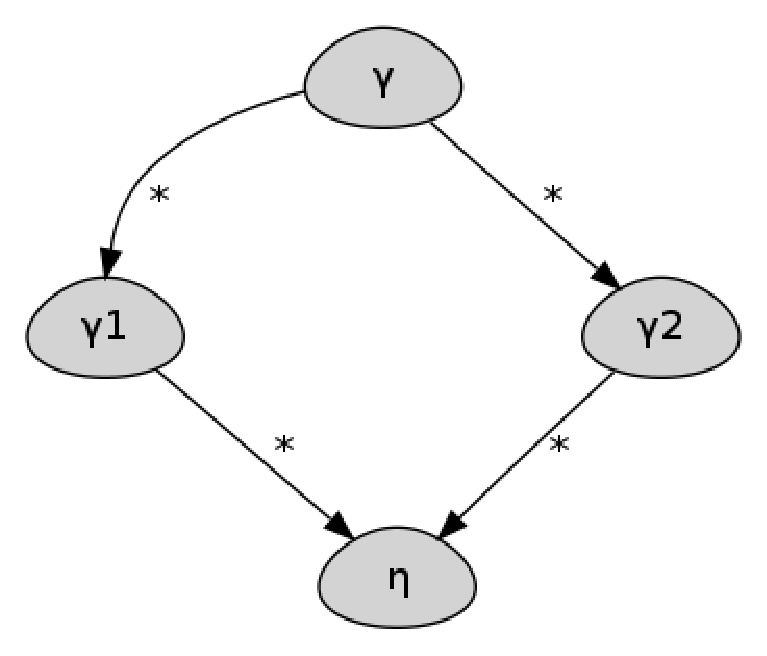
\includegraphics[height=0.3\textheight]{eps/konfluencia.eps}
  \end{center}
\end{figure}

Egy alapvet�en determinisztikus programoz�si nyelv szempontj�b�l
kritikus az, hogy minden helyes kifejez�s ki�rt�kel�se egy�rtelm�
eredm�nyt adjon, �gy az
egy�rtelm� norm�l forma, �s ennek kapcs�n a konfluencia k�v�natos
tulajdons�gok. Term �t�r� rendszerekn�l k�t fontos g�tja van a
konfluenci�nak; mivel ezek �ltal�nos�t�sai a gr�f�t�r� rendszerek, �gy
ezeket vizsg�ljuk meg el�sz�r.

\subsubsection{T�bb�rtelm�s�g}

A gr�f�t�r� rendszerek szab�lyait vizsg�ljuk ebben a r�szben. K�t
k�l�nb�z� szab�ly  $\alpha_1$ �s $\alpha_2$ bal oldalai \emph{teljesen
  �tfedik egym�st}, ha
l�tezik egy olyan adatgr�f, mely mindk�t baloldalnak
p�ld�nya. $\alpha_1$ �s $\alpha_2$ \emph{r�szlegesen �tfedik egym�st},
ha l�tezik egy olyan adatgr�f, mely $\alpha_1$-nek p�ld�nya,
$\alpha_2$ egy val�di (nem v�ltoz�) r�szgr�fj�nak p�ld�nya. K�t ilyen
r�szlegesen �tfed� bal oldalt \emph{kritikus p�r}nak is szokt�k
h�vni. A jobb oldalak f�ggv�ny�ben egy kritikus p�r okozhatja a t�bb
k�l�nb�z� norm�l forma l�tez�s�t is. Ciklikus strukt�r�kn�l az is
el�fordulhat, hogy egy r�szgr�f t�bbf�lek�ppen is illeszkedik
ugyanarra a r�szlegesen �tfed� szab�lyra.

\begin{pelda}
  A k�vetkez� p�lda a r�szleges �tfed�st mutatja be:

  \begin{shorthand}
    \con{f} (\con{g} $a$ 1) & 1 \\
    \con{g} $a$ $b$ & $a$
  \end{shorthand}

  A fenti �t�r� rendszerben a g 0 1 r�szgr�f nyilv�n egy redex, �s az
  els� szab�ly bal oldala egy nem v�ltoz� r�szgr�fj�nak p�ld�nya, �gy
  a k�t szab�ly r�szlegesen �tfedi egym�st. Ez azt jelenti, hogy
  p�ld�ul az f (g 0 1) adatgr�f reduk�lhat� f 0-ra vagy 1-re is.

  Egy p�lda arra, hogyan illeszkedhet t�bbf�lek�ppen is egy r�szgr�f a
  megfelel� r�szlegesen �tfed� szab�lyra:

  \begin{canonGRS}
    r:~\con{F}~x, \\
    x:~\con{F}~a &\rightarrow~~r \leftarrow a \\
    \\
    \cn{1}&:~\con{F}~\cn{2}, \\
    \cn{2}&:~\con{F}~\cn{1}
  \end{canonGRS}

  Figyelj�k meg, hogy az egyetlen szab�ly r�szlegesen �tfedi �nmag�t
  (a r�szleges �tfed�sn�l nem k�t�tt�k ki azt, hogy $\alpha_1 \not =
  \alpha_2$).
  Az als� adatgr�f k�tf�lek�ppen illeszkedik a fels� szab�lyra:
  egyr�szt $\mu(r) = \cn{1}$, $\mu(x) = \cn{2}$, $\mu(a) = \cn{1}$, m�sr�szt
  $\mu(r) = \cn{2}$, $\mu(x) = \cn{1}$, $\mu(a) = \cn{2}$.
\end{pelda}

Ez a t�bb�rtelm�s�g teh�t egy potenci�lis forr�sa a konfluencia
mentess�gnek, �gy ki kell k�sz�b�lni a jelens�get. Szerencs�re egy
trivi�lis m�dos�t�ssal ez megoldhat�, mely az �t�r� rendszerek
l�nyeg�n nem v�ltoztat. Rendelj�nk k�l�nb�z� priorit�sokat a
szab�lyokhoz, �s illeszt�sn�l mindig a legkisebb (vagy legnagyobb,
defin�ci� k�rd�se) priorit�s� szab�lyt pr�b�ljuk el�sz�r illeszteni. A
Haskell nyelvben p�ld�ul ezt a priorit�st egyszer�en a szab�lyok
sorrendje adja. Illeszt�sn�l mindig a forr�s sz�vegben el�bb szerepl�
szab�lyt vessz�k figyelembe el�sz�r.

\subsubsection{�sszehasonl�t�s}

Egy �t�r�si szab�ly bal oldala \emph{�sszehasonl�t�} akkor �s csak
akkor, ha l�tezik egy olyan v�ltoz� cs�cs azonos�t�, mely egyn�l
t�bbsz�r szerepel benne. Egy gr�f�t�r� rendszer \emph{�sszehasonl�t�}
akkor �s csak akkor, ha egy vagy t�bb szab�ly bal oldala
�sszehasonl�t�. Ekkor az illeszt�sn�l a cs�cs azonos�t�k egyenl�s�g�t
kell vizsg�lni (�sszehasonl�tani �ket), �s csak egyez�s eset�n
illeszkedhet a szab�ly. Ez sajnos a gyakorlatban nem haszn�lhat� j�l,
mivel csak egy szintaktikai azonoss�got vizsg�lunk, de adott esetben
el�fordulhat, hogy k�t r�szgr�f szintaktikailag nem, de szemantikailag
azonosak. A szemantikai azonoss�g viszont az �ltal�nos esetben sajnos
algoritmikusan nem eld�nthet�. Term�szetesen vannak olyan esetek,
amikor ez eld�nthet�, p�ld�ul amikor a gr�fok norm�l form�ban vannak
(ilyenkor a szintaktikai egyenl�s�g implik�lja a szemantikai
azonoss�got), de ez m�g nem el�g a gyakorlati haszn�lhat�s�g
szavatol�s�hoz. A mi szempontunkb�l megk�zel�tve, a Haskell nem engedi
meg a szab�lyok bal oldal�n a duplik�lt v�ltoz� el�fordul�st, �gy ez
nem vesz�lyezteti a konfluenci�t.

\begin{pelda}
  A k�vetkez� p�lda egy �sszehasonl�t� gr�f�t�r� rendszert mutat be:

  \begin{shorthand}
    \con{isEqual} $x$ $x$ & \con{True}\\
    \nl
    \con{Start} & \con{isEqual} $2$ ($1+1$)
  \end{shorthand}

  L�that�, hogy a start szimb�lumra nem illeszkedik az egyetlen
  szab�ly, mivel a k�t argumentum szintaktikailag nem azonos.
\end{pelda}

\subsubsection{�nmagukat be�gyaz� redexek �s a $\bot$}

Egy redex \emph{�nmag�t be�gyaz�}, ha a gy�ker�t mag�ra kell
ir�ny�tani. Form�lisan, l�teznie kell egy $\mu$ lek�pez�snek a $r :
\alpha \rightarrow \beta, \varphi$ szab�lyhoz �gy, hogy a megfelel�
$\mu''$ lek�pez�st alkalmazva a $\varphi = n \leftarrow m$ redirekci�
bal- �s jobb oldal�ra, ugyanazt a konstans cs�cs azonos�t�t kapjuk:
$\mu''(n) = \mu''(m)$. �gy az ilyen redexek �nmaguk reduk�ltjai. Az
al�bbi p�lda bemutatja, hogy okozhat ez konfluencia-mentess�get.

\begin{pelda}
  Legyenek a szab�lyaink a k�vetkez� alak�ak:

  \begin{shorthand}
    \con{A} $x$ & $x$ \\
    \con{B} $x$ & $x$
  \end{shorthand}

  Ekkor a k�vetkez� gr�f k�t redexet is tartalmaz:

  \begin{canonDG}
    \cn{1} & \con{G} \cn{2} \cn{3}, \\
    \cn{2} & \con{A} \cn{3}, \\
    \cn{3} & \con{B} \cn{2}
  \end{canonDG}

  Att�l f�gg�en, hogy el�sz�r \con{A} szerint vagy \con{B} szerint
  reduk�lunk, a redukci� ut�n m�r csak a m�sik szab�ly szerint tudunk
  reduk�lni, de ez viszont m�r �nmag�t be�gyaz� redexet eredm�nyez,
  melyet az �t�r�s helyben hagy. �gy teh�t a k�t norm�l form�ja a
  fenti adatgr�fnak:

  \begin{doubleDG}
    \multicolumn{2}{c}{El�sz�r \con{A} szerint reduk�lva} &
    \multicolumn{2}{c}{El�sz�r \con{B} szerint reduk�lva} \\
    \cn{1} & \con{G} \cn{3} \cn{3} & \cn{1} & \con{G} \cn{2} \cn{2} \\
    \cn{3} & \con{B} \cn{3}        & \cn{2} & \con{A} \cn{2}        \\
  \end{doubleDG}
\end{pelda}

Ennek a probl�m�nak az egyik megold�sa az, hogy bevezetj�k a speci�lis
$\bot$ konstans szimb�lumot, �s az �nmagukat be�gyaz� redexeket egy
kiv�teles esetk�nt kezelve az �t�r�si folyamat negyedik (�tir�ny�t�si)
l�p�s�ben erre a $\bot$-ra reduk�ljuk. Ezzel tulajdonk�ppen
defini�ltuk az �res cs�cs fogalm�t, melyet teh�t a $\bot$ szimb�lum
jelk�pez, �s angol neve \emph{bottom}. Ez a v�ltoztat�s egy�bk�nt utat
nyit a gr�f�t�r� rendszerek kateg�riaelm�leti t�rgyal�s�nak is, melyre
nyugodt sz�vvel mondhatjuk, hogy pozit�v eredm�ny.

\subsection{Megoszt�s}

A gr�f�t�r� rendszerek egyik jellegzetess�ge, ami az egyik oka a
kifejez�erej�knek a \emph{megoszt�s}. Ez annak a jelens�gnek a neve,
amikor a szab�lyok jobb oldal�n felhaszn�ljuk a m�r kisz�m�tott
eredm�nyeinket, ezzel elker�lve a sz�m�t�sok t�bbsz�r�z�s�t. A
megoszt�s (angolul \emph{sharing}) jellegzetess�ge, hogy a jobb
oldalon k�t vagy t�bb helyen ugyanaz a v�ltoz� cs�cs azonos�t�
szerepel. A k�vetkez� p�lda \told\acite{cleanbook}+bol{} sz�rmazik;
azt demonstr�lja, hogyan lehet sz�m�t�studom�nyi szempontb�l
``bonyolult'' p�ld�kat eleg�nsan megoldani ezzel a technik�val.

\begin{pelda}
  Ebben a p�ld�ban rendezett form�ban �ll�tjuk el� az �sszes $2^n3^m$
  alak� sz�mot, ahol $n \text{ �s } m \ge 0$. A megold�s Haskell-ben:

  \begin{lstlisting}
    hamm = let x = 1 : merge (map (*2) x) (map (*3) x) in x
    hamm' = ham' 1
        where
          ham' f = f : merge (ham' (f*2)) (ham' (f*3))

    merge []      []      = []
    merge f       []      = f
    merge []      s       = s
    merge f@(a:b) s@(c:d) = if a < c then
                                a : merge b s
                              else
                                if a == c then
                                   merge f d
                                else
                                   c : merge f d
  \end{lstlisting}

  Itt k�t k�l�nb�z� megold�st adtunk a probl�m�ra. Az els�
  (\emph{hamm}) megoszt�st haszn�l a m�r eddig kisz�molt listaelemek
  �jrahasznos�t�s�ra, a m�sodik (\emph{hamm'}) pedig explicit
  rekurzi�t. A megoszt�st haszn�l� megold�s polinomi�lis id�ben �s
  t�rhelyben fut, m�g a m�sik mindk�t szempontb�l exponenci�lis.
  A futtat�si eredm�nyeket mutatja a k�vetkez� (tipikus) GHCi kimenet:

  \begin{verbatim}
*Main> last $ take 200 hamm
15116544
(0.02 secs, 7377568 bytes)
*Main> last $ take 200 hamm'
15116544
(14.00 secs, 3187670248 bytes)
  \end{verbatim}

  Mindk�t verzi�val kisz�moltattuk a k�tsz�zadik elemet a
  sorozatban. Az eredm�ny term�szetesen ugyanaz a nyolc jegy� sz�m, de
  a rekurzi�s verzi�nak ehhez 14 m�sodpercre, �s k�r�lbel�l 3 gigabyte
  (!) mem�ria allok�l�s�ra volt sz�ks�ge, m�g a megoszt�sos technik�t
  haszn�l� v�ltozat mind�ssze k�t sz�zad m�sodperc alatt 7
  megabyte-nyi mem�ria allok�ci� mellett tudta ugyanezt az eredm�nyt
  produk�lni.

  �rdekess�gk�ppen megadjuk a k�t fajta implement�ci�hoz tartoz�
  adatgr�fok kanonikus alakj�t, illetve azok grafikus megjelen�t�s�t.

  \begin{doubleDG}
    \multicolumn{2}{c}{Megoszt�ssal} &
    \multicolumn{2}{c}{Rekurzi�val} \\
    \cn{1} & \con{Cons} 1 \cn{2} & \cn{1} & \con{Cons} 1 \cn{2} \\
    \cn{2} & \con{Merge} \cn{3} \cn{4} & \cn{2} & \con{Merge} \cn{3} \cn{4}\\
    \cn{3} & \con{Map} \cn{5} \cn{1} & \cn{3} & \con{Ham'} \cn{5} \\
    \cn{4} & \con{Map} \cn{6} \cn{1} & \cn{4} & \con{Ham'} \cn{6} \\
    \cn{5} & * \cn{7} & \cn{5} & * \cn{7} \cn{8} \\
    \cn{6} & * \cn{8} & \cn{6} & * \cn{7} \cn{9} \\
    \cn{7} & 2 & \cn{7} & 1 \\
    \cn{8} & 3 & \cn{8} & 2 \\
    \multicolumn{2}{c}{} & \cn{9} & 3
  \end{doubleDG}

  A k�l�nbs�g jobban l�tszik, ha �br�zoljuk a k�t adatgr�fot. Ahogy
  azt \aref{fig:hammrec} �s \aref{fig:hammshar} �br�k is mutatj�k, a
  rekurzi�s esetben is kialakul egy megoszt�s (nevezetesen a Haskell
  k�dban a \emph{ham'} f�ggv�ny \emph{f} param�ter�n, azaz az adatgr�f
  eset�ben a \cn{7} cs�cson), de ez nem ad l�nyeges gyors�t�st az
  algoritmusnak, m�g a m�sik verzi�n�l a megoszt�s m�g r�ad�sul
  ciklikuss� is teszi az adatgr�fot.

  \begin{figure}[hb]
    \captionsetup{position=top}
    \captionsetup[subfloat]{captionskip=-20pt}
    \caption{Hamming sz�mok list�j�nak adatgr�fjai}
    \begin{center}
      \subfloat[Hamming sz�mok rekurzi�val]{
        \label{fig:hammrec}
        \includegraphics[height=0.4\textheight]{eps/hamm_recurse.eps}
        \captionsetup{position=top}
      }
      \vrule
      \subfloat[Hamming sz�mok megoszt�ssal]{
        \captionsetup{position=top}
        \label{fig:hammshar}
        \hspace{1cm}
        \includegraphics[height=0.4\textheight]{eps/hamm_share.eps}
      }
      \vspace{0.5cm}
    \end{center}
    \label{fig:hamm}
  \end{figure}

  \begin{megj}
    A p�lda az egyszer�s�g kedv��rt nem sorolja fel az �sszes Hamming
    sz�mot, csak a kett�vel vagy h�rommal oszthat�kat. Az �sszes
    regul�ris sz�m felsorol�s�hoz egy h�rom param�teres \emph{merge}
    f�ggv�nyt kellene defini�lni, mely harmadik param�terben az �ttel
    is v�gig kellene szorozni a list�nkat. Ezt a feladatot az olvas�ra
    b�zzuk.
  \end{megj}

\end{pelda}

\section{Redukci�s strat�gi�k}

Legyen $\Theta$ a gr�f�t�r� rendszerek, $\Gamma$ pedig az adatgr�fok
halmaza. A $\sigma : \Theta \times \Gamma \rightarrow \Gamma$
f�ggv�nyt \emph{redukci�s strat�gi�}nak nevezz�k, ha adott $\rho \in
\Theta$ gr�f�t�r� rendszer �s $\gamma_0 \in \Gamma$ adatgr�f eset�n
$\forall \gamma \in \sigma(\rho, \gamma_0): \gamma \text{ redex }
\gamma_0\text{-ban } \rho\text{-ra n�zve}$. A $\sigma$ megadja, hogy
egy adott adatgr�f (�s �t�r� rendszer) eset�n melyik redexre hajtsunk
v�gre el�sz�r �t�r�si l�p�st. Ha $\exists \rho \in \Theta, \gamma_0
\in \Gamma : |\sigma(\rho, \gamma_0)| > 1$, akkor a $\sigma$ egy
nemdeterminisztikus redukci�s strat�gia. Ekkor tetsz�leges sorrendben
reduk�lhatjuk a $\sigma$ �ltal megadott redexeket. L�teznek olyan
redukci�s strat�gi�k, melyek t�bb redexet is megadnak p�rhuzamos
reduk�l�sra. Ezeket p�rhuzamos redukci�s strat�gi�knak h�vj�k, de
ebben a diplomamunk�ban ilyen t�pus�akkal nem foglalkozunk.

A \emph{reduk�l�} egy olyan folyamat, ami egy meghat�rozott strat�gia
szerint sorra reduk�lja a redexeket. A folyamat v�get �r, amint a
redukci�s strat�gia nem ad vissza reduk�lhat� redexet. Egy redukci�s
strat�gia \emph{normaliz�l�} akkor �s csak akkor, ha b�rmilyen
$\gamma$ adatgr�fra, melynek l�tezik norm�l form�ja, az a
reduk�l� folyamat, mely ezt a strat�gi�t k�veti �s $\gamma$-b�l indul,
norm�l form�val termin�l. Egy $\sigma$ redukci�s strat�gia
\emph{hipernormaliz�l�} akkor �s csak akkor, ha annak ellen�re, hogy
a $\sigma$-t�l \textbf{v�ges sz�m�} tetsz�leges redukci�s l�p�ssel
elt�r�nk, m�g mindig normaliz�l� marad. Ez a fogalom k�l�n�sen fontos
az eset�nkben, mert lehet�s�get ad p�r l�p�s erej�ig elt�rni a
szok�sos redukci�s strat�gi�t�l. Ez nagyon hasznos p�ld�ul
hiba-k�vet�s vagy optimaliz�l�s eset�n.

Sajnos nem l�tezik normaliz�l� strat�gia egy tetsz�leges gr�f�t�r�
rendszer eset�n, ez�rt csak olyan speci�lis, konfluens rendszereket
n�z�nk, melyek j�l viselkednek ebb�l a szempontb�l. T�bb �rdekes
oszt�lyuk van a gr�f�t�r� rendszereknek, egy r�sz�ket a termek
�t�r�s��rt felel�s rendszerekb�l lehet kieg�sz�teni gr�f�t�r�
rendszerekk�. Mi most egy ilyen oszt�lyt vizsg�lunk meg, de ehhez
el�bb egy speci�lis redukci�s strat�gi�t ismertet�nk.

\subsection{Funkcion�lis redukci�s strat�gia}

A \emph{funkcion�lis redukci�s strat�gia} c�lja egy egyszer�en
�tl�that�, de ugyanakkor hat�kony algoritmus meghat�roz�sa a redexek
ki�rt�kel�s�nek sorrendj�re. Ezt a strat�gi�t haszn�lja a legt�bb
funkcion�lis nyelv, pont az el�bbi k�t tulajdons�g miatt. Az
algoritmus a k�vetkez�: ha t�bb �t�r�si szab�ly van egy adott
f�ggv�nyre, a szab�lyokat a defini�l�suk sorrendj�ben ``fentr�l
lefel�'' pr�b�ljuk; a mint�kat ``balr�l jobbra'', sorrendben pr�b�ljuk
illeszteni; �s ha az aktu�lis argumentumnak egy nem-v�ltoz� mint�ra
kell illeszkednie, akkor ezt az argumentumot mindenk�ppen ki�rt�kelj�k
(\emph{a ki�rt�kel�s er�ltet�se})
mintailleszt�s el�tt (ez a folyamat r�szlegesen illeszked� szab�lyok
eset�n is). Ha a ki�rt�kel�s ut�n a mintailleszt�s sikeres, akkor
folytatjuk a k�vetkez� poz�ci�n tal�lhat� argumentummal eg�szen addig,
am�g az eg�sz szab�ly nem illeszkedik (vagy az egyik mintailleszt�s
nem siker�l). Amennyiben az egyik mintailleszt�s sikertelen, �gy
pr�b�ljuk a k�vetkez� szab�ly bal oldal�t illeszteni \textbf{az �gy
  kialakult kifejez�sre} (teh�t a ki�rt�kel�sek eredm�ny�t nem dobjuk
el). Ha egyik szab�lyt sem tudjuk alkalmazni, a gr�funk (er�s) gy�k�r
norm�l form�ban van. Amennyiben norm�l form�t k�vetel�nk meg a
strat�gi�t�l, �gy a kialakult gy�k�r norm�l form�k r�szgr�fjaira
rekurz�van alkalmazzuk a strat�gi�t.

A funkcion�lis redukci�s strat�gia teh�t egy gyakorlati kompromisszum
eredm�nye: hat�konyan implement�lhat�, �s a sz�m�t�sokat k�nnyen
�rthet�en lehet vele kifejezni. Tov�bbi el�nye, hogy k�nny�
elmagyar�zni a m�k�d�s�t, nem oper�l bonyolult fogalmakkal, k�nnyen
haszn�lhat� -- a szab�lyokhoz rendelt implicit priorit�s nagyon
hasonl�t a programoz�si nyelvekben szok�sos \emph{if \ldots then
  \ldots else} konstrukci�ra.

\section{Funkcion�lis gr�f�t�r� rendszerek}

A funkcion�lis gr�f�t�r� rendszerek alapjait a hasonl� nev�
funkcion�lis term �t�r� rendszerek kieg�sz�t�sek�nt kapjuk. �ltal�ban
az el�z� r�szben defini�lt funkcion�lis redukci�s strat�gia �rtelm�ben
priorit�sokat rendel�nk az egyes szab�lyokhoz; egy illeszked� szab�lyt
csak akkor v�laszthatunk a redukci�s l�p�shez, ha a magasabb
priorit�s� szab�lyok sosem fognak illeszkedni az (illeszt�s k�zben
esetleg m�dosult, �t�rt) adatgr�fra. Sajnos az �ltal�nos esetben
algoritmikusan nem eld�nthet� az, hogy egy gr�f valaha illeszkedni
fog-e egy adott mint�ra a bels� �t�r�sok k�vetkezm�nyek�nt, de a
ki�rt�kel�s er�ltet�se el�bb-ut�bb egy olyan helyzethez vezet, amiben
m�r ezt a k�rd�st el lehet d�nteni. Egyetlen probl�ma van ezzel az
er�ltet�ssel: ennek okak�nt elk�pzelhet�, hogy a ki�rt�kel�s sosem fog
termin�lni, pedig szemantikailag ez elker�lhet� lenne.

Ez a strat�gia a funkcion�lis gr�f�t�r� rendszerek l�nyeges t�bbs�g�re
normaliz�l�. Ha csak olyan elt�r� l�p�seket tesz�nk a strat�gi�t�l,
mely a priorit�si szab�lyoknak megfelel, akkor ez a redukci�s
strat�gia m�g hipernormaliz�l� is ezekre az �t�r� rendszerekre
(r�szletek�rt l�sd a k�vetkez�ket: \cite{cleanbook}, \cite{funcstrat})

%% Local Variables:
%% coding: latin-2
%% End:

% LocalWords:  CanonicalGRS Rule RedexPattern Contractum Redirection StartNode
% LocalWords:  ContractumPattern GraphRewriteSystem Nat Succ rule rwrredir bol
% LocalWords:  cleanbook isEqual let merge map in ham where if then else GHCi
% LocalWords:  hammrec hammshar position subfloat captionskip pt strat�gi�

\chapter{Implement�ci�}
\label{chap:impl}

Ebben a fejezetben a diplomamunk�hoz tartoz� program implement�ci�s
k�rd�seivel foglalkozunk.

\section{A program szerkezete}
A programot Haskell nyelven implement�ltuk, mivel egyr�szt mag�t a
forr�sk�dot k�nnyen lehet feldolgozni (sz�mos sz�vegfeldolgoz�
k�nyvt�rcsomag l�tezik ezen a nyelven; mivel a legn�pszer�bb Haskell
ford�t�t is Haskell-ben �rt�k, fel tudtuk haszn�lni az ebb�l sz�rmaz�
seg�df�ggv�nyeket a forr�sk�d elemz�s�hez), m�sr�szt a gr�f�t�r�
rendszer implement�l�sa is bonyodalommentesen t�rt�nt, k�sz�nhet�en a
nyelv st�lus�nak, mely k�zel �ll a matematikai formalizmus nyelv�hez.

A k�dot k�t nagy csoportra bonthatjuk: egy k�nyvt�rcsomagra �s a
felhaszn�l�i fel�letre. A felhaszn�l�i fel�let felel�s a param�terek
megfelel� beolvas�s��rt, a hib�k tov�bb�t�s��rt a felhaszn�l� fel�,
illetve term�szetesen a gr�fok kirajzol�s��rt.

\subsection{Felhaszn�l�i fel�let}
A fel�let k�dja egyr�szt a \emph{GraphRewrite/Main.hs} f�jlban
tal�lhat�, m�sr�szt a \emph{GraphRewrite/Main} k�nyvt�r f�jljaiban. A
program maga t�bbsz�l�; egy sz�l a megjelen�t�s�rt felel�s, egy m�sik
pedig mag�t a sz�m�t�st (a gr�f�t�r�st) v�gzi. A k�t sz�l k�z�tt a
kommunik�ci� egy szinkroniz�l� (k�z�s) v�ltoz�n kereszt�l t�rt�nik,
melyet a \emph{Control.Concurrent.MVar} csomag biztos�t. A gr�fok
kirajzol�s�hoz a \cite[GraphViz]{graphviz} programcsomagot
haszn�ltuk.

\subsection{K�nyvt�rcsomag}
A k�nyvt�rcsomag fel�lete a \emph{GraphRewrite.hs} f�jlban tal�lhat�,
mely val�j�ban csak �jra export�lja a \emph{GraphRewrite/Internal}
k�nyvt�r alatt tal�lhat� bels� modulok nyilv�nos fel�let�t. A
\emph{SimpleHaskell} modul egy saj�t, leegyszer�s�tett
reprezent�ci�j�t adja a Haskell nyelvnek. Erre az�rt volt sz�ks�g,
mert a \cite[GHC]{ghc}, a nyelv egyik legn�pszer�bb
ford�t�programj�nak r�szek�nt sz�ll�tott beolvas� k�nyvt�rcsomag
a gr�f�t�r� rendszerek szempontj�b�l t�l sok inform�ci�t
tartalmazott. A \emph{Convert} modul feladata az im�nti beolvas�s
eredm�ny�t a leegyszer�s�tett reprezent�ci�ra ford�tani. A feldolgoz�s
k�vetkez� f�zis�t a \emph{Rename} modul v�gzi, mely a beolvasott
program forr�s�ban a sz�veg azonos�t�kat kicser�li egyedi pozit�v
eg�sz sz�mokra (p�ld�ul a $sin a$ kifejez�sben a $sin$ f�ggv�ny
helyett az $1$, az $a$ v�ltoz� helyett pedig a $2$ sz�m azonos�t�t
�rja) �gy, hogy k�zben a l�that�s�gi szab�lyokat is figyelembe
veszi. Ezen ponton k�sz vagyunk a gr�f�t�r� rendszer l�trehoz�s�ra,
melyet a \emph{RewriteApp} modul hajt v�gre. Maga az �t�r� rendszer
strukt�r�ja �s a k�zvetlen�l hozz� tartoz� seg�df�ggv�nyek �s -t�pusok
a \emph{RewriteTypes} modulban ker�ltek defini�l�sra. Az �t�r�si
l�p�seket v�grehajt� f�ggv�nyeket a \emph{Rewrite} modulban
defini�ltuk.

A \ref{fig:arch} �bra mutatja a k�l�nb�z� modulok kapcsolat�t, azt a
folyamatot, ami egy Haskell forr�sf�jlb�l gr�f�t�r� rendszert
k�sz�t. A szaggatott vonal modulon bel�li inform�ci��raml�st jelent, a
t�bbi pedig k�t k�l�nb�z� modul k�z�tt mutatja ezt. Az \emph{AST}
mozaik sz� az ,,absztrakt szintaxisfa'' (angolul \emph{Abstract Syntax
  Tree}) r�vid�t�se, a \emph{Convert} modul ezt �ll�tja el�. A k�t
hatsz�ggel jel�lt cs�ccsal jel�lt m�veleteket a \emph{Rename} modul
v�gzi, valamint a v�gs� gr�f�t�r� rendszert a \emph{RewriteApp}
�ll�tja el�.

\begin{figure}[htb!]
  \begin{center}
    \includegraphics[width=16cm]{eps/arch.eps}
    \caption{A k�nyvt�rcsomag architekt�r�ja}
    \label{fig:arch}
  \end{center}
\end{figure}

Egy elk�sz�lt �t�r� rendszer seg�ts�g�vel hajthatunk csak v�gre
�t�r�si l�p�seket. �ltal�ban minden egyes kifejez�shez hozz�rendel�nk
egy (a term�szetes sz�mokon �rtelmezett) lek�pez�st, mely megadja a
kifejez�sben tal�lhat� referenci�k felold�s�t (ez teh�t egy $g : \N
\rightarrow \text{Kifejez�s}$ lek�pez�s). Az �gy kialakult p�rt h�vjuk
\emph{PointedGraph}-nak. A gr�f�t�r�st v�gz� \emph{rewriteStepFine}
f�ggv�nynek �gy sz�ks�ge van egy \emph{RewriteSystem} �s egy
\emph{PointedGraph} t�pusra, melyekb�l azt�n el��ll�tja az �t�r�si
l�p�seket tartalmaz� \emph{RewriteTree} f�t. Az�rt t�roljuk ezeket a
l�p�seket f�ban �s nem pedig list�ban, mert �gy �tl�that�bb az �t�r�si
l�p�sek szerkezete; egy �g egy r�szkifejez�s �t�r�s�nak felel meg.

\section{Navig�ci�}

Ahhoz, hogy a programban tudjunk az egyes �t�r�si l�p�sek k�z�tt
hat�konyan l�pkedni, valahogy el kell t�rolni az aktu�lisan
megjelen�tett l�p�st, valamint ahhoz, hogy visszafel� is tudjunk
l�pni (ak�r a kezd� kifejez�sig), az �sszeset ezen k�v�l is. Ez egy
tipikus esete az egy-f�kusz� adatszerkezeteknek, melyhez defini�lni
kell egy k�rnyezetet (\emph{Context}), �s egy adott �llapotot ekkor
a $(\textit{RewriteTree}, \textit{Context})$ p�r
reprezent�lja. A \cite{zipper} \emph{Zippers via Differentiation}
alpontja szerint a \emph{Context} t�pus�t �gy kapjuk, ha a
\emph{RewriteTree} t�pus�t deriv�ljuk.

Az al�bbiakban egy a \emph{RewriteTree}-n�l �ltal�nosabb fa
adatszerkezet t�pus�t deriv�ljuk, melyet a k�vetkez� Haskell k�ddal
�rhatunk le:
\begin{lstlisting}
  data Tree a = Branch a [Tree a]
\end{lstlisting}
A t�pusfunktor fel�r�s�hoz sz�ks�g�nk lesz egy szok�sosan defini�lt
lista t�pusra is:
\begin{lstlisting}
  data List a = Nil | Cons a (List a)
\end{lstlisting}
�gy m�r defini�lhatjuk a funktorainkat a k�vetkez�k�ppen:
\begin{eqnarray}
  \mathit{ListF}_AX &=& 1 + A \times X \nonumber\\
  \mathit{List} A &=& \mu X.\mathit{ListF}_AX \nonumber\\
  \mathit{TreeF}_AX &=& A \times \mu Y.\mathit{ListF}_X Y \nonumber\\
  \mathit{Tree} A &=& \mu X.\mathit{TreeF}_AX \nonumber
\end{eqnarray}
Mindenekel�tt sz�ks�g�nk lesz a lista funktor deriv�ltj�ra $A$
szerint:
\begin{eqnarray}
  \partial_A(\mathit{ListF}_AX) \cong X \label{math:listderiv}
\end{eqnarray}
A fa funktor deriv�ltj�hoz fel kell haszn�lnunk a k�vetkez�
(fixpontokra vonatkoz�) deriv�l�si szab�lyt: $\partial_X(\mu Y.F Y)
\cong \mu Y.F Y \times \partial_XF(\mu Y.F Y)$
\begin{eqnarray}
  \partial_X(\mathit{TreeF}_AX) &\cong& A \times \partial_X(\mu
  Y.\mathit{ListF}_X Y) \nonumber\\
  &\cong& A \times \mu Y.\mathit{ListF}_X Y \times
  \partial_X\mathit{ListF}_X(\mu Y.\mathit{ListF}_X Y) \nonumber
\end{eqnarray}
Ahova behelyettes�tve \told\ref{math:listderiv}+t{} kapjuk a k�vetkez�
azonoss�got:
$$ \partial_X(\mathit{TreeF}_AX) \cong A \times \mu Y.\mathit{ListF}_X
Y \times \mu Y.\mathit{ListF}_X Y $$
Ahol $X$ hely�re $\mathit{Tree} A$-t helyettes�tve:
$$ \partial\mathit{TreeF}_A(\mathit{Tree} A) \cong A \times
\mathit{List}(\mathit{Tree} A) \times \mathit{List}(\mathit{Tree}A) $$
Ahonnan \cite{zipper} szerint megkapjuk a k�rnyezetet:
$$ \mathit{Context}_{\mathit{Tree}_A} \cong \mathit{List}(A \times
\mathit{List}(\mathit{Tree} A) \times \mathit{List}(\mathit{Tree}A))$$
Ezt Haskellre ford�tva, �s $A$-nak a \emph{PointedGraph} t�pust
v�lasztva kapjuk a k�vetkez� (\emph{RewriteTypes} modulban
megtal�lhat�) t�pusdefin�ci�t:
\begin{lstlisting}
  type Context = [RewriteBranch]
  data RewriteBranch = RewriteBranch
      { node :: PointedGraph
      , left :: [RewriteTree]
      , rght :: [RewriteTree]
      }
\end{lstlisting}
Ekkor az aktu�lis �llapotot egy $(\mathit{RewriteTree},
\mathit{Context})$ p�rral �br�zoljuk. A \emph{Context}, illetve a
\emph{RewriteBranch} \emph{left} mez�je veremk�nt m�k�dik, teh�t az
aktu�lis cs�cshoz legk�zelebbi elem ker�l a lista elej�re. �gy amikor
m�lyebbre l�p�nk az adatszerkezetben, akkor az el�gaz�st hozz�f�zz�k a
\emph{Context} elej�hez; balra l�p�s eset�n a \emph{rght} komponens
elej�re f�zz�k (�s az �j aktu�lis elem a \emph{left} lista tetej�n
l�v� lesz); jobbra �s felfel� l�p�sn�l pedig szimmetrikusan. Egyb�l
l�tszik, hogy minden m�velet konstans l�p�ssz�mot ig�nyel, illetve
b�rmilyen r�szf�b�l kiindulva a n�gy elemi l�p�ssel (le, balra,
jobbra, fel) b�rmelyik r�szf�ba el tudunk jutni. Ez volt a c�lunk az
adatstrukt�ra bevezet�s�vel.

%% Local Variables:
%% coding: latin-2
%% End:

% LocalWords:  GraphRewrite GraphViz hs Internal SimpleHaskell GHC Convert Tree
% LocalWords:  Rename RewriteApp RewriteTypes Rewrite Abstract Syntax Context
% LocalWords:  PointedGraph rewriteStepFine RewriteSystem RewriteTree Zippers
% LocalWords:  via Differentiation n�l Branch List ListF AX TreeF XF type left
% LocalWords:  RewriteBranch rght

\chapter{Program dokument�ci�}

Ebben a fejezetben a diplomamunk�hoz tartoz� program felhaszn�l�i, �s
fejleszt�i dokument�ci�j�t ismertetj�k.

\section{Felhaszn�l�i dokument�ci�}

\subsection{Telep�t�s}

A program telep�t�se k�tf�lek�ppen t�rt�nhet: a \emph{cabal-install}
nev� csomagkezel�vel, vagy an�lk�l. A sikeres telep�t�shez a sz�ks�ges
Haskell csomagokat\footnote{A \emph{gtk}, a \emph{svgcairo} �s a
\emph{cairo} csomagok egy helyr�l, a gtk2hs projekt honlapj�r�l
let�lthet�ek:
\href{http://www.haskell.org/gtk2hs/}{http://www.haskell.org/gtk2hs/},
a t�bbi csomag
mind el�rhet� a HackageDB-r�l:
\href{http://hackage.haskell.org}{http://hackage.haskell.org}}
�s a minimum verzi� k�vetelm�nyeket \aref{tab:csomagok} t�bla mutatja.

\begin{table}[htb]
  \label{tab:csomagok}
  \begin{center}
    \begin{tabular}{| r | l |}
      \hline
      \bf csomag neve & \bf minimum verzi� \\
      \hline
      \hline
      base & 4.1.0.0 \\
      \hline
      containers & 0.2.0.0 \\
      \hline
      cabal & 1.6 \\
      \hline
      value-supply & 0.5 \\
      \hline
      lazysmallcheck & 0.3 \\
      \hline
      haskell-src & 1.0.1.2 \\
      \hline
      ipprint & 0.3 \\
      \hline
      fgl & 5.4.2.2 \\
      \hline
      pretty & 1.0.1.0 \\
      \hline
      graphviz & 2009.5.* \\
      \hline
      \hline
      strict-concurrency & 0.2.1 \\
      \hline
      parallel & 1.1.0.1 \\
      \hline
      directory & 1.0.0.3 \\
      \hline
      process & 1.0.1.1 \\
      \hline
      gtk & 0.10.0 \\
      svgcairo & 0.10.0 \\
      cairo & 0.10.0 \\
      \hline
    \end{tabular}
  \end{center}
  \caption{A sikeres telep�t�shez sz�ks�ges Haskell csomagok. Az als�
    r�szben lev� csomagok a futtathat� programhoz sz�ks�ges, a t�bbi
    pedig a k�nyvt�rcsomagokhoz is.}
\end{table}

\subsubsection{Telep�t�s \emph{cabal-install}-al}

A forr�sk�dot tartalmaz� k�nyvt�rba l�pve (ahol a
\tt{visual-graphrewrite.cabal} f�jl tal�lhat�) a k�vetkez� parancsot
kell kiadni:

\begin{verbatim}
cabal install
\end{verbatim}

\subsubsection{Telep�t�s \emph{cabal-install} n�lk�l}

A telep�t�s h�rom f� l�p�sb�l �ll. El�sz�r is a forr�sk�dot tartalmaz�
k�nyvt�rba l�pve (ahol a \tt{visual-graphrewrite.cabal} f�jl
tal�lhat�) a k�vetkez� parancsot kell kiadni:

\begin{verbatim}
runhaskell Setup.lhs configure
\end{verbatim}

Ez a parancs leellen�rzi a sz�ks�ges f�gg�s�gek megl�t�t, �s be�ll�tja
a ford�t�shoz sz�ks�ges param�tereket. A k�vetkez� parancs leford�tja
a forr�sk�dot, �s elk�sz�ti a linkelhet� k�nyvt�rcsomagokat �s a
futtathat� bin�rist:

\begin{verbatim}
runhaskell Setup.lhs build
\end{verbatim}

Ekkor m�r haszn�lhat� �llapotban van a program, azonban a megfelel�
helyre m�sol�shoz, telep�t�shez a sz�ks�ges jogosults�gok megszerz�se
ut�n a

\begin{verbatim}
runhaskell Setup.lhs install
\end{verbatim}

parancs futtat�sa sz�ks�ges.

\subsection{A program haszn�lata}

A futtathat� bin�ris alapesetben a \emph{visual-graphrewrite} nevet
kapja. Amennyiben ez el�rhet� a \tt{PATH} k�rnyezeti v�ltoz� egyik
k�nyvt�r�b�l, akkor a k�vetkez�k�ppen haszn�lhat�:

\begin{verbatim}
visual-graphrewrite modul.hs
\end{verbatim}

A parancssori argumentumokr�l egy r�vid �sszefoglal�t kapunk a
k�vetkez� parancs kiad�s�val (a k�vetkez� r�szlet mutatja a parancs
kimenet�t is):

\begin{verbatim}
$ visual-graphrewrite --help
visual-graphrewrite: unrecognized option `--help'
Usage: visual-graphrewrite [OPTION...] files...
  -v       --verbose      verbose output on stderr
  -d       --debug        show debug info on stdout
  -V, -?   --version      show version number
  -i FILE  --input=FILE   input FILE
  -m TERM  --main=TERM    main term on which to perform rewriting
\end{verbatim}

Az opci�k r�vid le�r�s�t \aref{tab:opciok} t�bl�zat tartalmazza. K�t
f� m�k�d�si m�dja van a programnak. Ha nincs megadva kezdeti
kifejez�s, ahonnan ind�thatn�nk az �t�r�st, akkor a szab�lyok jobb
oldalait jelen�ti meg. Ha megadtuk ezt a kifejez�st, akkor
term�szetesen az �t�r�si folyamatot elind�tja, �s az egyes l�p�seket
jelen�ti meg a k�perny�n. A bemeneti Haskell modul forr�s�t vagy a
standard bemeneten v�rja a program, vagy amennyiben megadunk egy
f�jlnevet, onnan beolvassa.

\begin{table}[htb]
  \begin{center}
    \begin{tabular}{|m{2.5cm}|m{6cm}||p{4cm}|}
      \hline
      \multicolumn{2}{|c||}{\bf Az opci� �s magyar�zata} & \bf P�lda a haszn�lat�ra \\
      \hline
      \hline
      \begin{verbatim}-v\end{verbatim} vagy \begin{verbatim}--verbose\end{verbatim} & Hiba eset�n r�szletesebb inform�ci�t �r a program a standard hiba kimenetre
      & \tt{visual-graphrewrite --verbose modul.hs} \\ \hline
      \begin{verbatim}-d\end{verbatim} vagy \begin{verbatim}--debug\end{verbatim} & R�szletesebb inform�ci�kat �r a program bels� m�k�d�s�r�l a standard kimenetre
      & \tt{visual-graphrewrite --debug modul.hs} \\ \hline
      \begin{verbatim}-V\end{verbatim} vagy \begin{verbatim}-?\end{verbatim} vagy \begin{verbatim}--version\end{verbatim} & A program ki�rja a verzi�j�t �s kil�p
      & \tt{visual-graphrewrite --version} \\ \hline
      \begin{verbatim}-i FILE\end{verbatim} vagy \begin{verbatim}--input=FILE\end{verbatim} vagy \begin{verbatim}FILE\end{verbatim}& FILE a bemenetk�nt funkcion�l� Haskell modul forr�sk�dj�t tartalmaz� f�jl neve. Ha nincs megadva, akkor a standard bemeneten v�rja a program a modul forr�s�t.
      & \tt{visual-graphrewrite --input=modul.hs} \\ \hline
      \begin{verbatim}-m TERM\end{verbatim} vagy \begin{verbatim}--main=TERM\end{verbatim} & TERM az �t�r�s kezdeti pontjak�nt �rtelmezett tetsz�leges Haskell kifejez�s
      & \tt{visual-graphrewrite --main='take 10 primes' --input=primes.hs} \\ \hline
      \hline
    \end{tabular}
  \end{center}
  \caption{A futtathat� program �ltal t�mogatott parancssori argumentumok le�r�sa.}
  \label{tab:opciok}
\end{table}

Ind�t�s ut�n a program megnyit egy ablakot, melyen a verzi�sz�m �s a
kezel�shez sz�ks�ges billenty�k eml�keztet�je tal�lhat�. Minden
esetben a megjelen�tett gr�fokat egy f�ba rendezve jelen�ti meg a
program, mindig csak egy gr�fot. A f�ban az aktu�lis cs�cs
legbaloldalabbi gyerek�re a \tt{d} billenty�vel l�phet�nk. Egy adott
cs�cs testv�rei k�z�tt jobbra a \tt{r}, balra a \tt{l} billenty�vel
v�logathatunk. Visszal�pni a sz�l� cs�csra a \tt{u} billenty�vel
lehet. Kil�p�shez a \tt{q} gombot kell megnyomni. K�nyelmi szempontb�l
hasznos a \tt{space} gomb, melynek funkcionalit�sa megegyezik a \tt{l}
billenty�j�vel, illetve a \tt{backspace}, mely a \tt{r} gombot
ut�nozza.

\section{Fejleszt�i dokument�ci�}

A k�nyvt�rcsomag fel�p�t�s�hez, �s az egyes modulok �ttekint�s�hez
sz�ks�ges inform�ci� megtal�lhat� \aref{chap:impl} fejezetben. A
program k�nyvt�rcsomagk�nt val� haszn�lat�hoz el�g import�lni a
\emph{GraphRewrite} modult, amely �jraexport�lja a nyilv�nosan
haszn�lhat� f�ggv�nyeket, adatt�pusokat.

A \emph{Language.Haskell.Parser} modul �ltal produk�lt
\emph{ParseResult} t�pusb�l egyszer�en tudunk leegyszer�s�tett
reprezent�ci�j� Haskell modult csin�lni a \emph{convParse}
f�ggv�nnyell. Az ennek eredm�nyek�ppen kapott modult a \emph{rename}
f�ggv�ny �ttranszform�lja �gy, hogy a sz�veg azonos�t�k hely�re
mindenhol egyedi sz�mokat �r, illetve visszaadja a sz�veg
$\rightarrow$ sz�m �sszekapcsol�sokat is. Ezekb�l a
\emph{makeRewriteSystem} f�ggv�ny egy gr�f�t�r� rendszert k�sz�t,
melyet azt�n felhaszn�lhatunk az �t�r�shoz. Magukat a redukci�s
l�p�seket a \emph{rewriteStepFine} f�ggv�ny seg�ts�g�vel lehet
elv�gezni, melynek meg kell adni egy kezd� kifejez�st is, �s visszaad
egy f�t az �t�r�si l�p�sekkel.

A k�vetkez� k�dr�szlet egy olyan esetet mutat be, melyben egy konstans
sz�vegben tal�lhat� Haskell modulb�l k�sz�t�nk gr�f�t�r� rendszert:

\begin{verbatim}
predef = map snd deltaNames
sup = unsafePerformIO newEnumSupply :: Supply Int
(ids, ids2, ids3) = split3 sup

(Ok (predefBinds,_,_)) = distributeIds predef ids2

m = parseModule "result = f 1; f 5 = 5; f a = f (succ a)"
renamed = rename' predefBinds (convParse m) ids3
(Ok (n,sm)) = renamed
rs = makeRewriteSystem sm n
\end{verbatim}

A \emph{distributeIds} f�ggv�ny a $\delta$-f�ggv�nyekhez rendel
azonos�t�kat ugyan�gy, mint ahogy a rename f�ggv�ny a modulokn�l.

%% Local Variables:
%% coding: latin-2
%% End:


\appendix
%%\include{cd_tartalma}
\newcommand{\tit}{\textsl}
\newcommand{\vol}{\textbf}

\begin{thebibliography}{00}
\bibitem{interm}Barendregt H.P., Eekelen M.C.J.D. van, Glauert J.R.W,
  Kennaway J.R., Plasmeijer M.J. and Sleep M.R.: \tit{Towards an
    intermediate language based on graph rewriting}, Proc. Parallel
  Architectures and Languages Europe, \vol{259}, 1987, [159--175].
\bibitem{cleanbook}M.J. Plasmeijer and M.C.J.D van Eekelen:
  \tit{Functional Programming and Parallel Graph Rewriting},
  Addison-Wesley, 1993, [113--181].
\bibitem{funcstrat}Toyama Y., Smetsers J.E.W., Eekelen M.C.J.D. van
  and Plasmeijer M.J.: \tit{The functional strategy and transitive
    term rewriting systems}, Term Graph Rewriting, John Wiley, 1993.
\bibitem{semantics}Marko C.J.D. van Eekelen and Sjaak Smetsers and
  Marinus J. Plasmeijer: \tit{Graph Rewriting Semantics for
    Functional Programming Languages}, CSL '96: Selected Papers from
  the 10th International Workshop on Computer Science Logic, 1997,
  Springer-Verlag, [106--128].
\bibitem{graphviz}AT\&T Research, Graphviz contributors: \tit{Graphviz
  - Graph Visualization Software}, Version 2.22, 10 March 2009. Link:
  \url{http://www.graphviz.org} (el�r�s d�tuma: 2009. m�rcius 10.)
\bibitem{ghc}Simon Marlow, Simon Peyton Jones, The GHC Team:
  \tit{The Glorious Glasgow Haskell Compiler}, Version 6.10.2, 1 April
  2009. Link: \url{http://haskell.org/ghc} (el�r�s d�tuma: 2009.m�jus
  20.)
\bibitem{zipper}Wikibooks, the open-content textbooks collection
  \tit{Haskell/Zippers}, 15 March 2009. Link:
  \url{http://en.wikibooks.org/wiki/Haskell/Zippers} (el�r�s d�tuma:
  2009. m�jus 26.)

\end{thebibliography}

\addcontentsline{toc}{chapter}{Irodalomjegyz�k}

%% Local Variables:
%% coding: latin-2
%% End:


\listoffigures

\end{document}

%% Local Variables:
%% coding: latin-2
%% End:
